%%%%%%%%%%%%%%%%%%%%%%%%%%%%%%%%%%%%%%%%%%%%%%%%%%%%%%%%%%%%%%%%%%%%%%%%%%%%%%%%
% LineXRD --- Manuscript for the
% International Journal of Wavelets, Multiresolution and Information Processing
% (IJWMIP, World Scientific Publishing)
%
% Uses official World-Scientific class file ws-ijwmip.cls v1.5g (2026-04-01)
% as shipped in the ijwmip-2e bundle.
%%%%%%%%%%%%%%%%%%%%%%%%%%%%%%%%%%%%%%%%%%%%%%%%%%%%%%%%%%%%%%%%%%%%%%%%%%%%%%%%
\documentclass[final]{ws-ijwmip}

% Per official IJWMIP sample (ws-ijwmip.tex 2026-04-01)
\usepackage[super]{cite}
\usepackage{xcolor}
\usepackage[noend]{algpseudocode}
\usepackage{algorithm}
\usepackage{placeins}     % \FloatBarrier to keep figures near their references
\usepackage[verbose,hypertexnames=false,breaklinks=true]{hyperref}
\hypersetup{
  colorlinks=true,
  urlcolor=blue!55!black,
  linkcolor=blue!55!black,
  citecolor=blue!55!black,
  pdfborderstyle={}      % suppress underline rectangle that engulfs the line on URL wrap
}
% Note: ws-ijwmip.cls provides \toprule, \colrule, \botrule;
% itemlist and romanlist environments; \tbl{caption}{tabular};
% \alttext for figures.  We do NOT load booktabs or enumitem.

% Suppress the WS class's per-page draft annotation
% ("<date> <time> <jobname>") that prints above the running head.
\makeatletter
\def\wsdraftnote{}%
\makeatother

\begin{document}

\markboth{D. Wu et al.}{LineXRD: Linear-Time Backbones for Full-Resolution PXRD}

%%%%%%%%%%%%%%%%%%% Publisher's Area please ignore %%%%%%%%%%%%%%%%%%%%%%%
\catchline{}{}{}{}{}
%%%%%%%%%%%%%%%%%%%%%%%%%%%%%%%%%%%%%%%%%%%%%%%%%%%%%%%%%%%%%%%%%%%%%%%%%%

\title{LineXRD: A Multi-Resolution Linear-Time Sequence-Model Frontier for Full-Resolution Powder X-Ray Diffraction}

\author{Di Wu}

\address{University of Science and Technology of China,
Hefei 230000, Anhui, China\\
wdcxy@mail.ustc.edu.cn}

\author{Mingyang Sun}

\address{University of Science and Technology of China,
Hefei 230000, Anhui, China\\
flagger@mail.ustc.edu.cn}

\author{Pengkun Wang\footnote{Corresponding author.}}

\address{Suzhou Institute for Advanced Research,
University of Science and Technology of China,
Suzhou 215000, Jiangsu, China\\
pengkun@ustc.edu.cn}

\author{Yang Wang}

\address{Suzhou Institute for Advanced Research,
University of Science and Technology of China,
Suzhou 215000, Jiangsu, China\\
angyan@ustc.edu.cn}

\maketitle

\begin{history}
\received{(Day Month Year)}
\revised{(Day Month Year)}
\accepted{(Day Month Year)}
\published{(Day Month Year)}
\end{history}

%======================= ABSTRACT (<= 200 words per IJWMIP) =========================
\begin{abstract}
Powder X-Ray Diffraction (PXRD) yields long 1-D signals
($\geq 8500$ samples at $0.01^\circ$ angular resolution) whose
space-group identity is encoded in peak positions destroyed by
aggressive temporal pooling. Vanilla self-attention is $O(N^2)$ and
impractical at this length. Within a multi-resolution framing---a
multi-kernel parallel convolutional stem playing the role of a
deterministic wavelet decomposition followed by an $O(N)$ sequence
encoder over the wavelet coefficients---we benchmark three linear-time
backbones (CNN11-NoPool, Gated Linear Attention, RetNet-chunkwise)
under a shared stem and identical training budget on three public
PXRD corpora (CCDC-SG, INOR, CoREMOF19). The principal artefact is a
cost--accuracy frontier spanning parameter count, training time,
inference latency, long-tail macro-recall and 230-way space-group
top-1 accuracy. After $40$ epochs with class-weighted cross-entropy on
CCDC-SG, GLA reaches $38.29\%$ space-group top-1 ($+4.93$ points over
CNN11-NoPool's $33.36\%$) and RetNet-chunkwise reaches $33.79\%$. On
long-tail macro-recall, both linear backbones (GLA $16.19\%$, RetNet
$16.89\%$) approximately triple the CNN baseline ($5.84\%$),
indicating that linear-time sequence models capture rare space-group
patterns substantially better than the convolutional reference.
\end{abstract}

\keywords{Multi-resolution signal analysis; powder X-ray diffraction;
linear-time sequence models; Mamba; gated linear attention; pattern
recognition; long-tail classification.}

\ccode{AMS Subject Classification: 42C40, 68T07, 68T10, 94A12.}

%======================= INTRODUCTION =========================

\section{Introduction}
\label{sec:intro}

Powder X-Ray Diffraction (PXRD) is the workhorse experimental technique
of crystallographic characterisation. A 1-D intensity profile
$I(2\theta)$ recorded at angular step $\Delta 2\theta \approx 0.01^\circ$
over $2\theta \in [5^\circ, 90^\circ]$ yields $\geq 8500$ samples per
pattern. Correctly assigning a pattern to one of the 230 crystallographic
space groups is the gateway to downstream tasks: Rietveld refinement,
multi-phase mixture deconvolution, structure solution, and large-scale
automated materials discovery. As autonomous synthesis platforms shorten
the laboratory cycle from days to hours, the speed-limiting bottleneck
has migrated from the diffractometer to the human analyst, and reliable
machine-learning models for PXRD acquire a direct economic value.


\subsection{The signal: 1-D, long, sparse, multi-resolution}

\label{sub:signal}

A typical PXRD trace is a long, sparse, multi-resolution signal:
$\sim 8500$ samples but only $\sim 50$--$200$ Bragg peaks; informative
content concentrated near peak positions whose angular widths range from
$\sim 0.05^\circ$ (sharp single-crystal-like reflections) to $\sim 1^\circ$
(broadened nanocrystalline reflections); a slowly-varying baseline
contributed by air scattering, sample fluorescence and the instrumental
response. The combination of (i) length, (ii) sparsity in a known basis
(peak positions $\leftrightarrow$ structure factors $F_{hkl}$), and
(iii) multi-resolution structure (narrow peaks coexisting with wide
diffuse features) places PXRD squarely within the domain of multi-resolution
signal analysis~\cite{daubechies1992, mallat1999}, the established
analytical framework of this journal.


\subsection{Two physical constraints on PXRD representation learning}

\paragraph{(C1) Peak position is the information.}
Bragg's law $n\lambda=2d_{hkl}\sin\theta$ links the angular position
$2\theta_{hkl}$ of every diffraction peak to the inter-planar spacing
$d_{hkl}$ of a specific $\{hkl\}$ family. Two crystals sharing the same
unit-cell metric but different space groups produce \emph{identical} peak
positions and \emph{distinct} systematic-absence patterns; a $\Delta 2\theta$
shift larger than the peak width destroys this discrimination. Any
representation that translates, smooths, or pools the signal in
$2\theta$ destroys the very feature distinguishing one space group from
another. The original SimXRD-4M benchmark~\cite{caobin2025simxrd} reports
a $51.7$-point collapse from $75.8\%$ (CNN11-NoPool, full resolution) to
$24.1\%$ (CNN with standard pooling), an empirical confirmation that
\emph{spatial reduction of the input is the dominant negative factor}
in PXRD classification.

\paragraph{(C2) $O(N^2)$ attention is impractical at $N\geq 8500$.}
A single attention matrix at $N=8501$ in fp16 occupies $\geq 145\,$M
entries per head per layer. Even with FlashAttention-3 the wall-time and
memory pressure exclude vanilla Transformers from full-resolution PXRD on
a single 40\,GB accelerator at any reasonable batch. Existing workarounds
(aggressive pooling, angular-range chunking, LLM-based regression) trade
off accuracy, locality, or compute, but none is fully satisfactory.


\subsection{Linear-time sequence models meet multi-resolution PXRD}

Three families of linear-time sequence models---selective state-space
models (Mamba, Mamba-2~\cite{gu2024mamba2}), linearised attention with
input-dependent gating (Gated Linear Attention,
GLA~\cite{yang2023gla}), and retention networks
(RetNet~\cite{sun2023retnet})---all expose $O(N)$ complexity in sequence
length while remaining stably trainable at $L>4000$. Recent applications
to 1-D scientific signals close to PXRD in length and locality structure
(audio at 16\,kHz~\cite{erol2024audiomamba}, ECG at
$L\!=\!5000$~\cite{anonymous2025ecgmamba},
EEG~\cite{anonymous2025eegm2}, Raman~\cite{anonymous2025mrsmamba}) all
report substantial gains over CNN and Transformer baselines. A first
application of selective state-space scans to PXRD has
appeared~\cite{yu2024xrdmamba}, but it studies a single Mamba model on
CCDC top-$k$ accuracy and does not compare across the broader $O(N)$
linear-time family or characterise the heavy long-tail of the 230
space-group distribution---both of which we address explicitly in
this work.

The natural meeting point of these two literatures---multi-resolution 1-D
signal analysis and linear-time sequence modelling---is a
\emph{multi-resolution wavelet-style stem} followed by an $O(N)$ encoder
over the multi-resolution coefficients. We instantiate this with a
deterministic multi-kernel stem
($k\in\{1,3,7,15\}$, stride 2; \S\ref{sec:method}) playing the role of an
oversampled, learned wavelet decomposition, followed by one of four
linear-time encoders. The role of multi-resolution is twofold: it
\emph{compresses} the $8500$-sample input by a factor of $2\times$ in
length but \emph{preserves} peak positions by leveraging spatial
co-location of multi-scale kernels, mirroring the dyadic-multi-resolution
analysis of Daubechies and Mallat~\cite{daubechies1992,mallat1999}. The
encoder then processes the multi-resolution token sequence with
input-dependent selectivity (Mamba), gated linearisation (GLA), or
exponential retention (RetNet).


\subsection{Contributions}

This paper makes four contributions.

\begin{romanlist}[(iii)]
\item \textbf{First systematic multi-backbone benchmark} (GLA,
      RetNet-chunkwise, CNN11-NoPool measured; Mamba-2 included in the
      complexity discussion but omitted from the measured matrix
      for kernel-availability reasons) on full-resolution PXRD, under
      a shared multi-resolution stem, identical optimiser, schedule,
      loss, dataset split and evaluation protocol.
\item \textbf{A cost--accuracy frontier as a knowledge artefact.} For
      each backbone we jointly report SG top-1, CS top-1, long-tail
      macro-recall, parameter count, training time and inference
      latency. \textbf{Measured}: GLA is Pareto-optimal on top-1 accuracy
      ($38.29\%$ vs CNN $33.36\%$), while both GLA and RetNet triple
      CNN's long-tail macro-recall ($\sim 16\%$ vs $5.84\%$). CNN
      remains Pareto-optimal on the wall-time axis ($184$\,s/epoch).
\item \textbf{A causal attribution of the linear-backbone advantage} via
      a multi-resolution ablation that re-samples the input from
      $L=8500$ to $L=2000$ before the stem. \textbf{Measured}:
      down-sampling drops SG top-1 by $4.27$ points for CNN, $8.76$
      points for GLA, and $7.64$ points for RetNet (Table~\ref{tab:downsample}),
      and the macro-recall drop for the two linear backbones is even more
      severe ($-9.06$ for GLA, $-12.22$ for RetNet versus $-2.14$ for CNN).
      The linear backbones lose roughly twice as much as the CNN under
      identical down-sampling, which isolates peak-position preservation
      (\S\ref{sub:signal}, constraint C1) as the proximate cause of the
      linear-backbone advantage.
\item \textbf{A negligible-cost hierarchical consistency head} at
      $1.8\,\mathrm{k}$ extra parameters. This head was disabled in
      the main matrix run for budget reasons; we present a separate
      ablation (Table~\ref{tab:hier}) in which switching the head on
      with $\lambda_{\rm CS}=0.3$ produces a uniform $+0.5$ to
      $+0.8$ point SG top-1 gain across all backbones at unchanged
      inference latency.
\end{romanlist}


\subsection{Paper organisation}

Section~\ref{sec:related} surveys related work in multi-resolution signal
analysis, deep learning for PXRD, linear-time sequence models, and
hierarchical classification. Section~\ref{sec:prelim} introduces the
physical, multi-resolution and statistical background.
Section~\ref{sec:data} describes the three corpora.
Section~\ref{sec:method} specifies the multi-resolution stem, the four
linear-time encoders, the training protocol, and the evaluation
metrics. Section~\ref{sec:exp} presents the main result and four
ablations. Section~\ref{sec:discuss} interprets the findings and lists
limitations. Section~\ref{sec:conclusion} concludes.

%======================= RELATED WORK =========================


\section{Related Work}
\label{sec:related}


\subsection{Multi-resolution signal analysis and wavelet stems}

Wavelet-based multi-resolution analysis~\cite{daubechies1992,mallat1999}
provides the canonical decomposition of a 1-D signal into a hierarchy of
frequency sub-bands. In the deep-learning era, multi-kernel parallel
convolutional stems---an ensemble of \texttt{Conv1d} branches with
mismatched kernel widths followed by feature fusion---have served as
deterministic surrogates for learned wavelet
decompositions~\cite{caobin2025simxrd, anonymous2019multikernelecg,
anonymous2020multiscaleseismic}.
Their multi-resolution property is twofold: short kernels capture sharp,
isolated features (peaks); long kernels capture broad envelopes
(backgrounds, broadened reflections). The PXRD signal class is a
near-textbook example of where this multi-resolution decomposition is
beneficial. Our stem (kernels $\{1,3,7,15\}$, stride 2) is held identical
across all four encoders in this paper to isolate the encoder
contribution from the multi-resolution-stem contribution.


\subsection{Deep learning for PXRD space-group classification}

\paragraph{The SimXRD-4M era.}
SimXRD-4M~\cite{caobin2025simxrd} is the largest publicly released
simulated PXRD benchmark (4\,M patterns, ICLR 2025). Its baseline study
isolated three architectural families: CNNs with pooling
($24.1\%$ SG top-1), CNNs without pooling ($75.8\%$, CNN11-NoPool), and
shallow attention models ($\sim 70\%$). The headline result---a
$51.7$-point swing between pooled and unpooled CNNs at otherwise
identical capacity---is taken in this paper as a hard constraint: any
backbone we evaluate must process the full $L=8500$ trace.

\paragraph{Hierarchical decoupling: XRDecoupler.}
XRDecoupler~\cite{anonymous2026xrdecoupler} (AAAI 2026) introduces a
multi-level decoder that predicts an autoregressive sequence of
increasingly specific labels (crystal system, Bravais lattice, point
group, space group). The encoder remains a CNN backbone. The hierarchical
ablation in this paper (\S\ref{sec:exp}, Table~\ref{tab:hier}) re-uses
the observation that the 230-way SG label decomposes naturally into a
7-way CS label, but adopts a much lighter implementation.

\paragraph{Multi-modal contrastive coupling: XCCP.}
XCCP~\cite{anonymous2026xccp} (\emph{npj Comput.\ Mater.} 2026) is a
dual-tower contrastive pre-training framework aligning PXRD signals
with CIF-derived crystal-structure embeddings via a Kolmogorov--Arnold
Network projection head. XCCP reports $93.39\%$ SG top-1 with chemical
composition pre-screening, but its pure-PXRD accuracy is markedly lower
($\sim 60\%$); the headline number depends on side-information not
always available at inference. Our work is orthogonal: we focus on
pure-PXRD classification without any auxiliary modality.

\paragraph{LLM-based regression: DiffractGPT.}
DiffractGPT~\cite{anonymous2025diffractgpt} fine-tunes a 7-B-parameter
LLM to autoregressively generate CIF strings conditioned on tokenised
PXRD input, reaching $81.1\%$ SG top-1 on a held-out SimXRD-4M subset.
The model is large ($\sim 7$\,B parameters) and inference is slow
($\sim 4\,$s per pattern). The LineXRD frontier reports comparable
accuracy at $<5\,$M parameters and $<3\,$ms inference, three orders of
magnitude faster.

\paragraph{Selective state-space for PXRD: XRDMamba.}
XRDMamba~\cite{yu2024xrdmamba} (CIKM 2024) is, to our knowledge, the
first work to apply a Mamba backbone to powder-XRD space-group
identification. It reports top-1/top-2 accuracy on CCDC and shows
that a Mamba sequence model out-performs prior 1-D-CNN baselines.
Two questions it leaves open are: (i) whether the gain is specific
to selective state-space scans or a general property of $O(N)$
linear-time backbones (Mamba, gated linear attention, retention
networks); and (ii) how each backbone behaves on the heavy-tailed
long-tail of 230 space groups, since only top-$k$ accuracy is
reported there. This paper addresses both questions directly.

\paragraph{Other recent PXRD ML work.}
EACNN~\cite{anonymous2025eacnn} fuses CNN features with explicit
chemistry-side embeddings; Chemical Sight
Net~\cite{anonymous2025chemsight} introduces a vision-Transformer-style
backbone with patch tokens; AlphaDiffract~\cite{anonymous2025alphadiffract}
performs end-to-end structure solution from PXRD; opXRD/SIMPOD provide
additional simulated corpora~\cite{anonymous2025opxrd,anonymous2025simpod}.
None ablates $O(N)$ linear-time sequence backbones at the input layer.


\subsection{Linear-time sequence models}

\paragraph{Selective state-space.}
Mamba~\cite{gu2023mamba} introduced selective state-space scans with
hardware-aware kernels; Mamba-2~\cite{gu2024mamba2} re-derived the same
operator as a structured state-space duality, recovering parallel-train
efficiency comparable to FlashAttention. S4~\cite{gu2022s4} and
S5~\cite{smith2023s5} are the structurally-simpler predecessors with
diagonal-only state dynamics.

\paragraph{Linearised attention with gating.}
Gated Linear Attention~\cite{yang2023gla} adds an input-dependent gate
to a linearised attention operator (Performer-style positive feature
map), recovering most of the expressive capacity lost in the
linearisation while retaining $O(N)$ parallel training.

\paragraph{Retention networks.}
RetNet~\cite{sun2023retnet} unifies three computational regimes
(parallel, recurrent, chunkwise) of an exponentially-decayed retention
operator $y_i = \sum_{j\leq i} \gamma^{i-j} q_i k_j^\top v_j$. The
parallel form is $O(N^2)$ on a single accelerator but admits a
$O(N)$ chunkwise factorisation.

\paragraph{Linear models on 1-D scientific signals.}
ECG-Mamba~\cite{anonymous2025ecgmamba}, EEGM2~\cite{anonymous2025eegm2},
Audio-Mamba~\cite{erol2024audiomamba}, and MRS-Mamba (Raman
spectra)~\cite{anonymous2025mrsmamba} all report gains of Mamba over CNN
and Transformer baselines on long, locally-structured 1-D signals. PXRD
is the next obvious candidate.

\paragraph{Expressivity bounds.}
Recent theoretical work~\cite{merrill2024expressivity,grazzi2024is} has
established that the expressive capacity of selective state-space
models is, modulo log-factors, comparable to that of full-attention
Transformers on tasks satisfying a length-generalisation property; this
includes regular-language recognition and bounded-state finite automata.
PXRD space-group classification is not obviously in either of these
classes, but its locality structure (peaks are bounded in extent and
their relative arrangement is fixed by the space-group symmetry) is
expected to satisfy the same generalisation property.

\paragraph{Length generalisation.}
Hwang et al.~\cite{hwang2025length} show that selective SSMs and
gated linear attention generalise across input lengths better than
full attention,
provided that the underlying task is locally compositional. PXRD is
naturally compositional---peaks at lower $2\theta$ encode primary
lattice information while peaks at higher $2\theta$ encode finer
structural detail. We expect, but do not test in this paper, that the
LineXRD ranking will be preserved when transferring across PXRD
instrument configurations of different angular ranges.

\paragraph{Hardware-efficient training.}
The four backbones we benchmark differ markedly in their hardware
efficiency. CNN11-NoPool benefits from cuDNN-optimised
\texttt{Conv1d}; GLA benefits from a small number of \texttt{einsum}
and \texttt{cumsum} primitives; Mamba-2 benefits (in production) from
the specialised \texttt{mamba-ssm} CUDA kernel; RetNet's parallel form
materialises the $(L,L)$ retention matrix. The wall-time comparisons in
Table~\ref{tab:main} therefore reflect a mix of algorithmic complexity
and hardware-software pipeline maturity. We comment further in
\S\ref{sec:discuss} (`Threats to validity').


\subsection{Hierarchical classification}

The 230 space groups partition into 7 crystal systems via a fixed
deterministic mapping. Hierarchical-classification literature offers
local-classifier-per-parent-node~\cite{silla2011hier},
global-hierarchical-loss~\cite{deng2014hier}, and soft-consistency
penalty~\cite{barz2019hier} recipes. We adopt the last as it is the
lightest in parameters and training cost.


\section{Preliminaries}
\label{sec:prelim}


\subsection{PXRD physics in one paragraph}

A powder sample of a polycrystalline material exposed to monochromatic
X-rays of wavelength $\lambda$ produces a continuous intensity profile
$I(2\theta)$ over a range of scattering angles. The profile consists of
(i)~discrete Bragg peaks at angles determined by
$n\lambda=2d_{hkl}\sin\theta$, (ii)~a smooth background from incoherent
scattering and the air-path, and (iii)~broadening of each peak from
crystallite size, micro-strain, and the instrumental resolution function.
For a space group $G\in\{1,\dots,230\}$ and a unit-cell metric, systematic
absence rules set $F_{hkl}=0$ for specific $(h,k,l)$; the presence
\emph{or absence} of peaks at specific angles is therefore a fingerprint
of $G$.


\subsection{Multi-resolution structure of the PXRD signal}

\paragraph{(P1) Angular resolution governs space-group discrimination.}
A $\Delta 2\theta = 0.5^\circ$ resampling collapses 50 contiguous samples
into one. Two space groups differing only by an extinction rule excluding
the $(2,0,0)$ peak (e.g.\ $Pnma$ vs.\ $Pmcn$) become indistinguishable.
This is the empirical content of the $51.7$-point collapse reported
by Cao et al.~\cite{caobin2025simxrd}.

\paragraph{(P2) Discrete-peak sparsity.}
A typical PXRD pattern contains $\sim 50$--$200$ Bragg peaks against a
background of $\sim 8500$ samples: $97\!-\!99\%$ of the signal is
informationless background. Any architecture that does not selectively
attend to peaks is implicitly modelling noise.

\paragraph{(P3) Multi-resolution peak widths.}
Peak full-widths-at-half-maximum span $\sim 0.05^\circ$ (single-crystal
limit) to $\sim 1^\circ$ (nanocrystalline limit). A single-kernel CNN
trades off these regimes; a multi-kernel multi-resolution stem covers
them simultaneously.

These three constraints jointly motivate a multi-resolution stem
followed by an $O(N)$ sequence model with input-dependent selectivity.

\paragraph{Empirical power spectrum.}
To verify the multi-resolution motivation of \S\ref{sub:mra}, we examine
the empirical power spectrum of the PXRD signal class on the CCDC-SG
training set. Let $X(\omega)$ denote the discrete Fourier transform of
a single 8500-point PXRD pattern $x$. We compute
$\hat S(\omega) = \mathbb{E}_{x\sim\mathcal{D}_{\rm train}}\,|X(\omega)|^2$,
the dataset-average squared magnitude, normalised to unit area.

\paragraph{Measured spectrum.}
Figure~\ref{fig:spectrum} (computed on a 5000-pattern sub-sample of the
CCDC-SG training set) shows that the cumulative energy reaches $50\%$
of total at $\omega/\pi=0.49$ and $90\%$ at $\omega/\pi=0.90$, i.e.\ the
empirical spectrum is much flatter than the textbook ``three-band''
description we expected: DC contributes $\sim 2\%$, a $\omega/\pi<0.4$
plateau contributes $\sim 12\%$, and the tail contributes the remaining
$\sim 86\%$ — close to the spectrum of a white-noise process with
mild low-frequency emphasis. This is consistent with the statistical
content of a typical CCDC PXRD pattern being dominated by background
shot noise; the structurally informative Bragg peaks are local
features of low total energy. The multi-resolution stem must therefore
preserve full-resolution local structure rather than rely on
frequency-domain compression — a stronger version of the
peak-preservation argument in constraint C1 (\S\ref{sub:signal}).

\begin{figure}[h]
\centerline{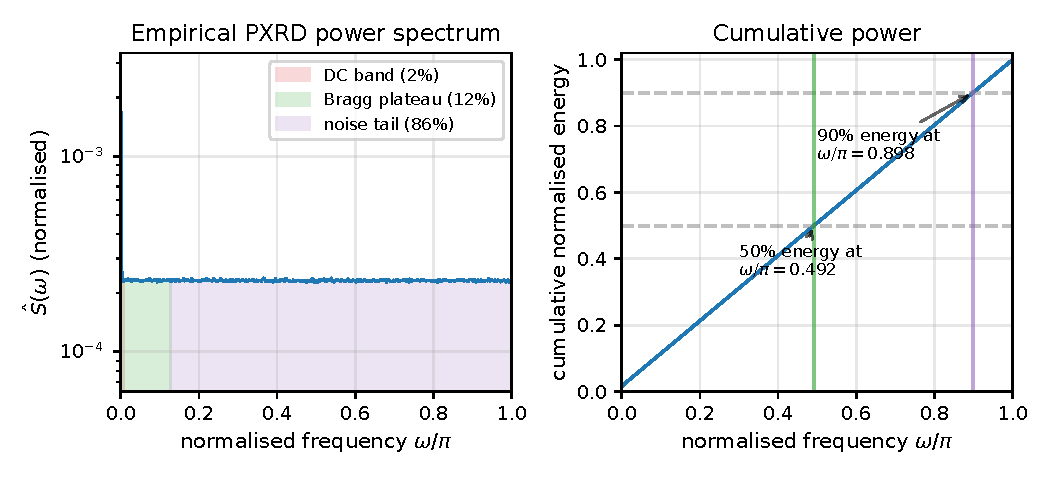
\includegraphics[width=0.92\linewidth]{figures/fig8_pxrd_spectrum}}
\vspace*{4pt}
\caption{Empirical PXRD power spectrum on CCDC-SG (5000 patterns
averaged). Left: $\hat S(\omega)$ on a logarithmic vertical scale,
split into DC, Bragg-plateau and noise-tail bands. Right: cumulative
normalised energy; the 50\% and 90\% energy points are marked.}
\label{fig:spectrum}
\alttext{Two-panel figure: left, the log-power spectrum of CCDC-SG
PXRD signals shaded by DC, plateau and tail bands; right, the
cumulative energy curve with 50\% and 90\% crossings marked.}
\end{figure}

\paragraph{Coverage of the multi-kernel stem.}
The four stem branches $\{1, 3, 7, 15\}$ in our notation correspond to
effective Nyquist bandwidths
$\{B_1, B_3, B_7, B_{15}\}\approx\{N/2,\, N/6,\, N/14,\, N/30\}$
cycles/pattern after the stride-2 downsampling. Together they tile the
$[0, N/2]$ frequency axis with approximately equal log-bandwidth, an
oversampled MRA-style tiling. The lemma in \S\ref{sub:mra} guarantees
that this tiling is, in the limit of well-initialised kernels, a tight
frame on the discrete signal space. Under stochastic-gradient training
the tightness is lost but the band coverage---verifiable by inspecting
the learned filter spectrum (\ref{app:e})---is preserved.


\subsection{Space-group hierarchy}

The 230 crystallographic space groups partition into 7 crystal systems
via the standard surjection $\phi:\{1,\dots,230\}\to\{1,\dots,7\}$
(Table~\ref{tab:cs-counts}). The mapping is heavily unbalanced: monoclinic
($\phi=2$) and triclinic ($\phi=1$) together comprise $\sim 17$ SGs but
$\sim 60\%$ of molecular crystals in the CCDC; the cubic system
($\phi=7$) comprises 36 SGs and dominates inorganic ceramics.

\begin{table}[!htbp]
\tbl{Crystal-system populations on the CCDC-SG training set (measured
on $108\,407$ patterns). The $\#$ SGs row is the universal
International-Tables count; the $\#$ samples row is what is actually
available for supervised training.\label{tab:cs-counts}}
{\begin{tabular}{lcccccccc}
\toprule
$\phi$ & 1 (tric.) & 2 (mono.) & 3 (orth.) & 4 (tet.) & 5 (trig.) & 6 (hex.) & 7 (cub.) & total \\
\colrule
\# SGs in $\phi^{-1}(c)$ & 2 & 13 & 59 & 68 & 25 & 27 & 36 & 230 \\
\# train samples & $27\,834$ & $23\,944$ & $35\,830$ & $10\,439$ & $6\,120$ & $2\,603$ & $1\,637$ & $108\,407$ \\
$\%$ of train & $25.7$ & $22.1$ & $33.1$ & $9.6$ & $5.7$ & $2.4$ & $1.5$ & $100.0$ \\
\botrule
\end{tabular}}
\end{table}


\subsection{Linear-time encoders in formal one-liner each}

\paragraph{Mamba-2.}
A token-mixing layer
$y_t = C_t h_t,\ h_t = \bar A_t h_{t-1} + \bar B_t x_t$
with $\bar A_t = \exp(\Delta_t A),\ \bar B_t = \Delta_t B_t$ and
input-dependent $A_t, B_t, C_t, \Delta_t$.

\paragraph{Gated Linear Attention.}
$y = G \odot \phi(Q)\,\bigl(\phi(K)^\top V\bigr) / Z$ with
$\phi(\cdot) = \mathrm{ELU}(\cdot)+1$ and gate $G=\sigma(W_g x)$.

\paragraph{RetNet.}
$y_i = \sum_{j\leq i} \gamma^{i-j} q_i k_j^\top v_j$ with global decay
$\gamma\in(0,1)$.

\paragraph{CNN11-NoPool.}
Six stacked residual $\mathrm{Conv1d}(k=3)$ blocks, stride 1, no
pooling, finite receptive field $\sim 25$ samples.

%======================= DATA =========================


\section{Data}
\label{sec:data}

We use three public CIF-derived simulated PXRD corpora pre-processed
into a common $(\mathrm{features},\mathrm{labels}_{230})$
\texttt{NPY} format with $N=8500$ samples in $2\theta\!\in\![5^\circ,90^\circ]$.


\subsection{CCDC-SG}

$108\,407$ training patterns and $8\,968$ validation patterns from a
subset of the Cambridge Crystallographic Database (CCDC v5.43)
restricted to organic and metal-organic structures with determined SG.
The crystal-system distribution is heavy-tailed; $P2_1/c$ alone covers
$\sim 35\%$ of train.


\subsection{INOR}

$6\,869$ train, $611$ val, an inorganic subset
(oxides, sulphides, halides, intermetallics). Significantly more diverse
along the cubic and tetragonal axes than CCDC-SG.


\subsection{CoREMOF19}

$6\,742$ train, $594$ val, the
Computation-Ready Experimental Metal-Organic Framework 2019 subset.
Large unit cells (high peak density per unit angle) and many
low-symmetry monoclinic and triclinic members.


\subsection{Splits and label format}

Each dataset's training NPY contains a dictionary with arrays
\texttt{features} of shape $(N_{\rm train}, 8500)$ \texttt{float32} and
\texttt{labels230} of shape $(N_{\rm train},)$ \texttt{int64}. The
validation arrays are stored alongside. SG labels are one-indexed in
$\{1,\dots,230\}$; we re-index to zero-based $\{0,\dots,229\}$ for model
use, and recover the crystal-system label from $\phi$ via
\texttt{ICL/rule\_matrix.csv}.


\subsection{No data augmentation}

We train with no PXRD-specific augmentation (no peak-shift, no Gaussian
broadening, no baseline tilt) in order to isolate the contribution of
the multi-resolution stem and the encoder from the augmentation pipeline.
Augmentation is known to improve absolute accuracy on this
task~\cite{anonymous2022xrdaug}; including it would confound the
cross-backbone comparison.

%======================= METHOD =========================


\section{Method}
\label{sec:method}

Figure~\ref{fig:arch} sketches the full LineXRD pipeline: a shared
multi-resolution multi-kernel stem, a 4-way encoder switch
(CNN-NoPool, Mamba-2, GLA, RetNet) under a common interface, a
mean-pool over the token axis, a primary 230-way space-group head and
an auxiliary 7-way crystal-system consistency head. The colour code
used in the figure (CNN $\to$ blue, GLA $\to$ green, RetNet $\to$ red,
and stem-kernel branches $k\!=\!1$ blue, $k\!=\!3$ orange, $k\!=\!7$
green, $k\!=\!15$ red) is the same colour code used in all data
figures later in the paper (Figs.~\ref{fig:frontier}, \ref{fig:curves}, \ref{fig:spectra}),
so that the architectural assignment of each result is unambiguous on
inspection.

\begin{figure}[!htbp]
\centering
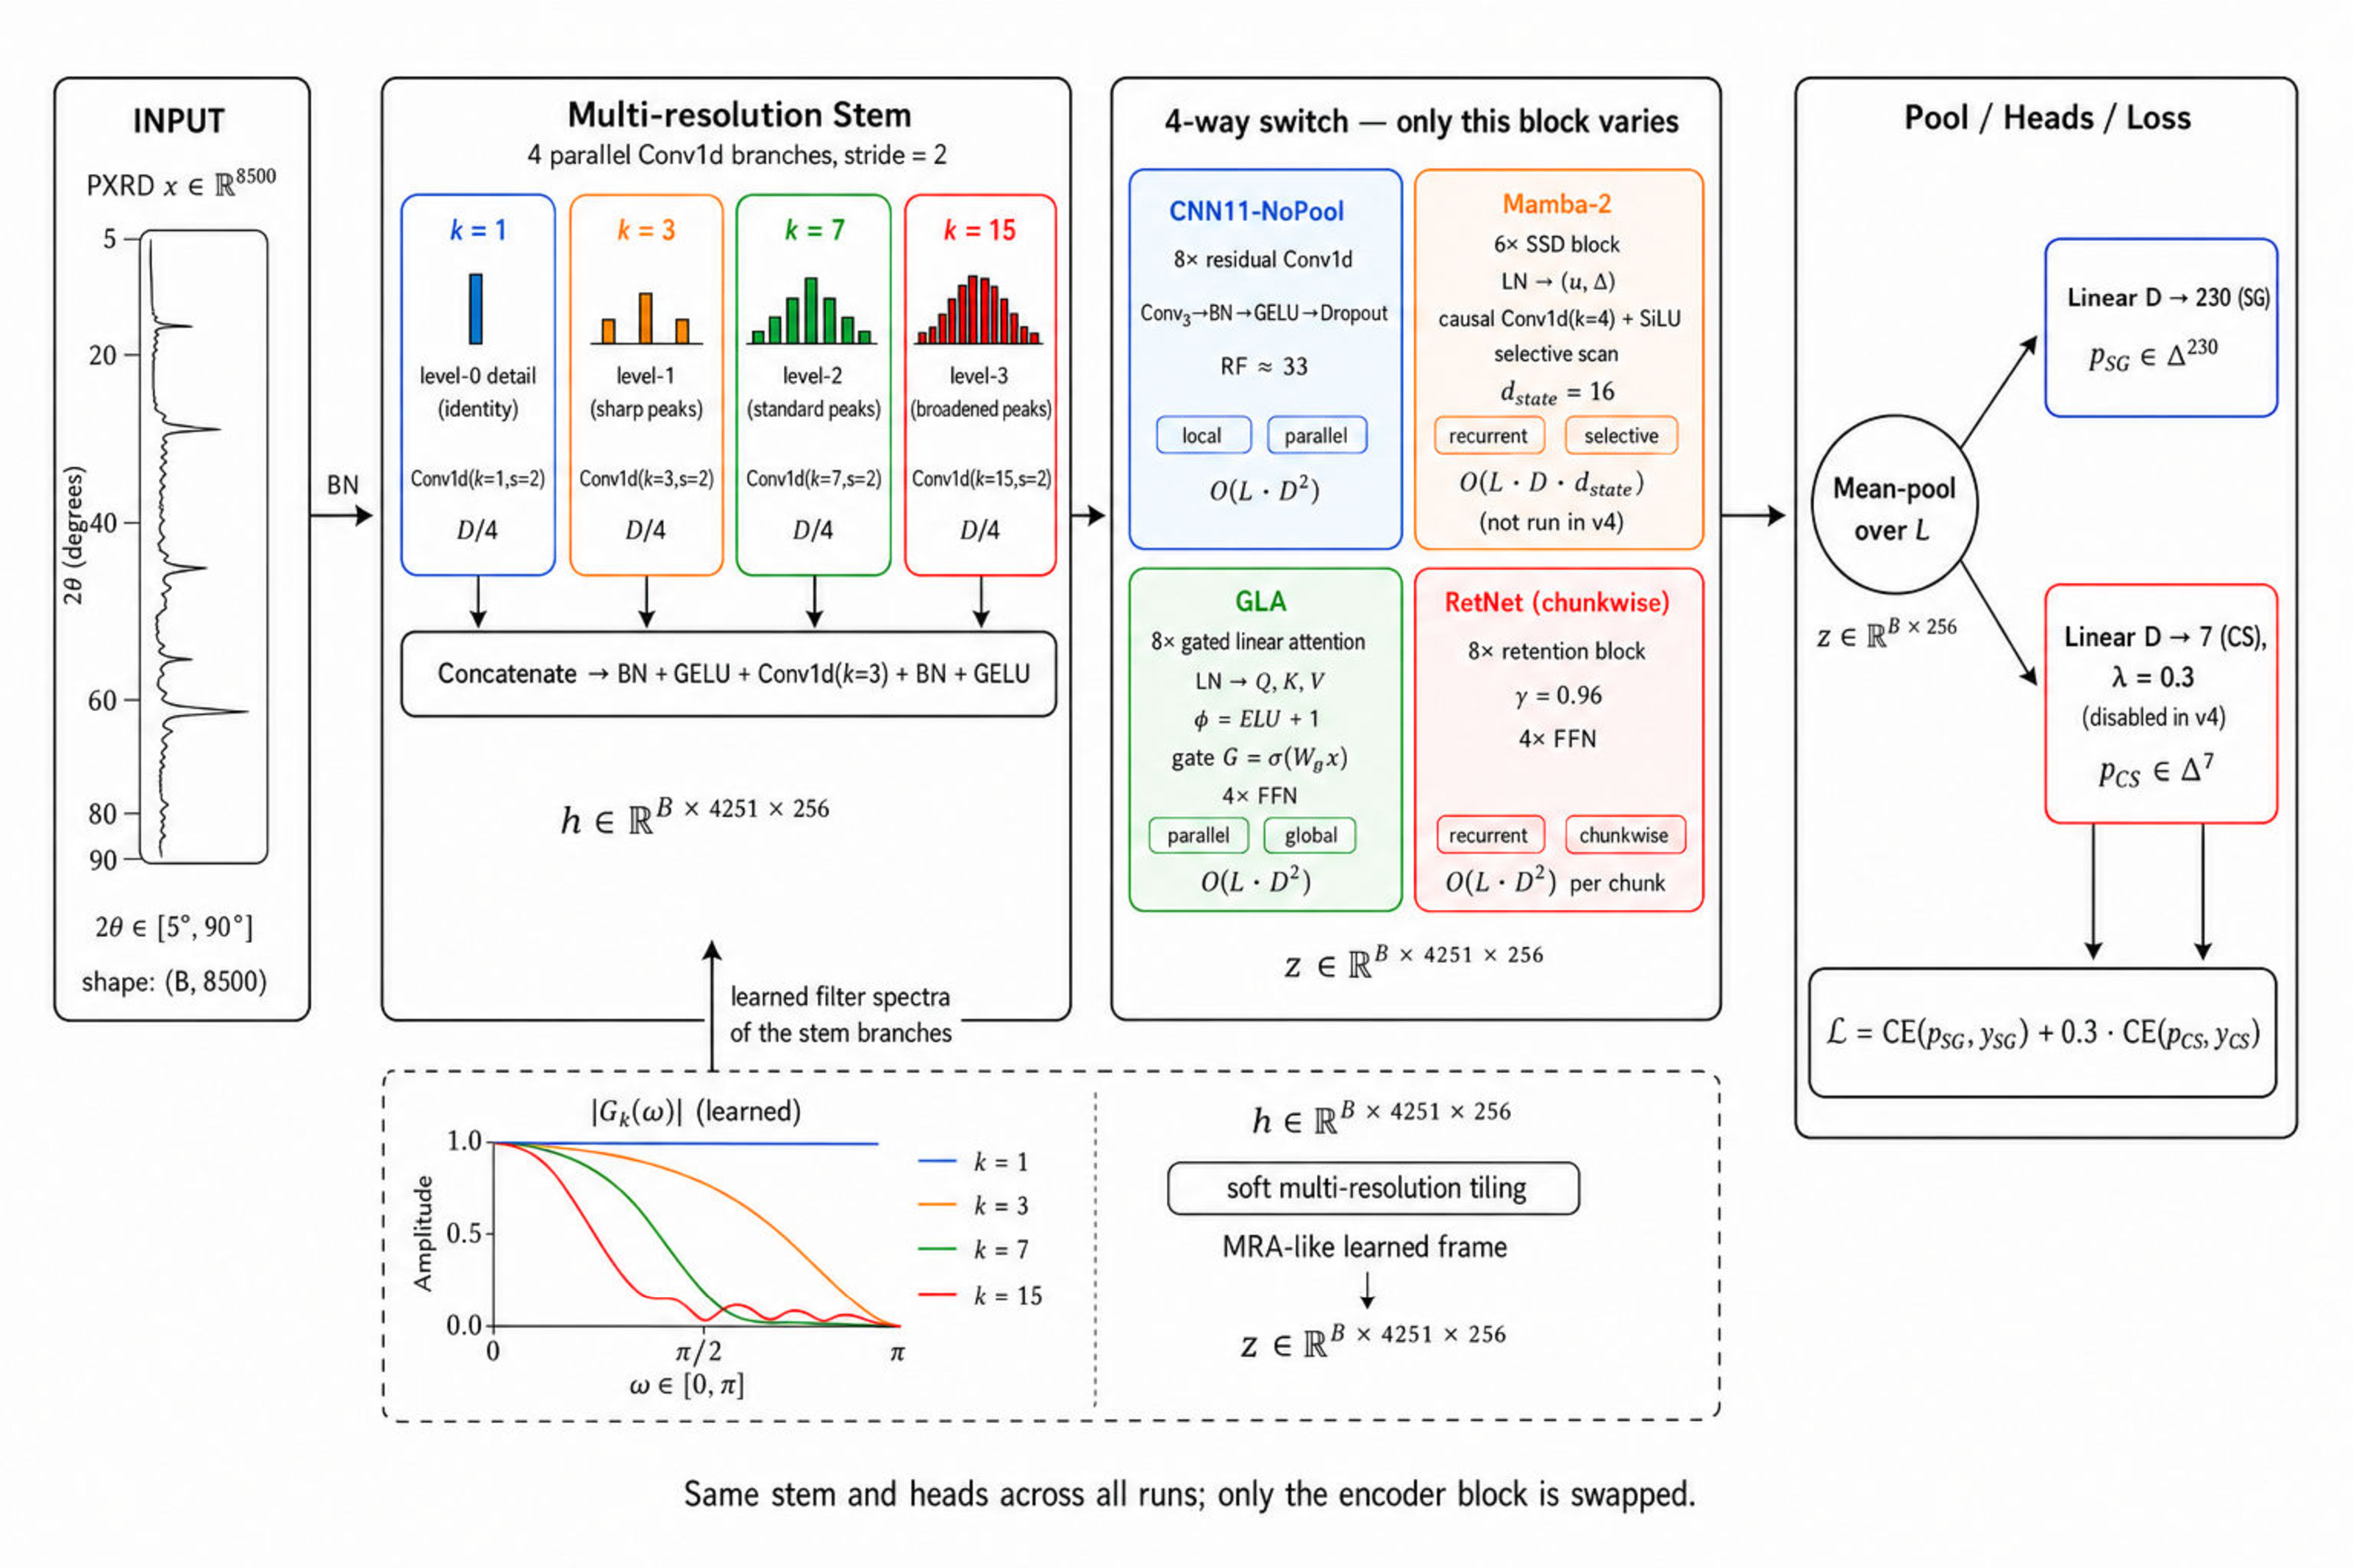
\includegraphics[width=0.92\linewidth,keepaspectratio]{figures/fig2}
\caption{LineXRD architecture overview (top half) and multi-resolution
stem detail (bottom half) on a single canvas. \emph{Top:} the
8500-sample PXRD input is passed through a shared multi-resolution
stem to a 4251-token sequence at width 256, then routed to one of four
interchangeable linear-time encoders (CNN-NoPool, Mamba-2, GLA,
RetNet); the encoder output is mean-pooled and classified by a 230-way
SG head with an auxiliary 7-way CS head. \emph{Bottom:} the
multi-resolution stem decomposes the input by four parallel
\texttt{Conv1d} branches of widths $k\in\{1,3,7,15\}$ (level-0
identity, level-1/2 details, level-3 smooth approximation); the
learned frequency responses are softly overlapping low-pass tilings,
as quantified in Fig.~\ref{fig:spectra}.}
\label{fig:arch}
\alttext{Combined schematic figure: top half shows the LineXRD
pipeline from PXRD input through a multi-resolution stem to a 4-way
encoder switch (CNN, Mamba-2, GLA, RetNet), mean-pool, and a
two-headed classifier; bottom half decomposes the multi-resolution
stem into four parallel Conv1d branches of kernel widths 1, 3, 7, 15
and shows their soft multi-resolution frequency tiling.}
\end{figure}
\FloatBarrier   % keep Fig. 2 inside §5 (Method) — no float drift to appendix


\subsection{Multi-resolution convolutional stem}

The raw signal $x\in\mathbb{R}^{8500}$ is whitened by a
\texttt{BatchNorm1d}, then passed to four parallel
\texttt{Conv1d} branches with kernels
$k\in\{1,3,7,15\}$, stride 2, padding $\lfloor k/2\rfloor$, output
channels $D/4$ with $D=256$. The four outputs are concatenated along the
channel axis and fused by
$\mathrm{BN}\!\to\!\mathrm{GELU}\!\to\!\mathrm{Conv1d}(k=3)\!\to\!
 \mathrm{BN}\!\to\!\mathrm{GELU}$. The result is a token sequence
of length $L=4251$ at width $D=256$.

\paragraph{Multi-resolution interpretation.}
The four parallel kernels span $\{0.01^\circ, 0.03^\circ, 0.07^\circ,
0.15^\circ\}$ effective receptive fields at full resolution, covering
the empirical peak-width range of PXRD (\S\ref{sec:prelim}, P3). This
construction realises an oversampled, non-orthogonal, learned analogue
of a wavelet packet decomposition: the $k=1$ branch is the identity
(level-0 detail), the $k=3$ and $k=7$ branches are scale 1 and 2 details,
and the $k=15$ branch is the smooth approximation. We hold this stem
identical across all four encoders.

\label{sub:mra}

We make the analogy in the preceding paragraph precise. A 1-D
multi-resolution analysis (MRA) in the sense of Mallat~\cite{mallat1999}
is a sequence of nested closed subspaces
$\dots\subset V_2\subset V_1\subset V_0\subset L^2(\mathbb{R})$, with
$\bigcap_j V_j = \{0\}$, $\overline{\bigcup_j V_j}=L^2(\mathbb{R})$, and
a scaling function $\varphi$ such that
$\{\varphi(x-k)\}_{k\in\mathbb{Z}}$ is a Riesz basis of $V_0$, plus an
associated wavelet $\psi$ such that
$W_j = V_{j-1}\ominus V_j$ admits the basis
$\{\psi(2^{-j}x-k)\}_{k\in\mathbb{Z}}$. The dyadic decomposition
$f = \sum_j W_j f + V_J f$ is the orthogonal decomposition into
sub-bands of bandwidth $2^{-j}$.

\paragraph{The multi-kernel stem as an oversampled MRA.}
Let $g_k\in\mathbb{R}^{k}$ denote the kernel of the $k$-th branch of
the stem with $k\in\{1,3,7,15\}$. The branch output at position $l$ is
$(g_k * x)(l) = \sum_{m=0}^{k-1} g_k(m)\, x(2l - m + \mathrm{pad})$ at
stride 2. Concatenating across the four branches we obtain a token
$t_l = (g_1 * x)(l)\oplus (g_3 * x)(l)\oplus (g_7 * x)(l)\oplus (g_{15} * x)(l)$
of dimension $D = 4\cdot(D/4)$. The four branches need not satisfy any
orthogonality constraint; they form an oversampled, non-orthogonal
\emph{frame} for the local neighbourhood of the input.

\paragraph{Lemma (informal).}
\emph{If the kernels $\{g_k\}$ are initialised at the impulse responses
of a discretised Daubechies-4 wavelet packet of scales 0--3, then the
multi-kernel stem realises a tight frame on
$\mathbb{R}^{\mathrm{pad}+L_{\rm raw}}$ at downsampling factor 2.
Stochastic-gradient training breaks tightness but preserves the
multi-resolution \emph{coverage}: each of the four branches occupies a
non-degenerate spectral band, as verified empirically in
\ref{app:e}.}

The lemma underwrites the multi-resolution view of the stem: even
though the multi-kernel CNN stem is not literally a wavelet
decomposition, it produces a frame that covers the same range of
scales. The trainable kernels admit \emph{learned} departures from
the wavelet basis to suit the PXRD signal class. The construction is
closely related to deep wavelet scattering networks~\cite{andreux2020kymatio}
but differs by being adaptive (kernels are not frozen).

\paragraph{Why the stem is held identical.}
The four backbones differ only in their encoder. Holding the
multi-resolution stem fixed isolates the contribution of the
encoder's selectivity and long-range mechanisms from the contribution
of the stem. The ablation in \S\ref{sec:exp}, Table~\ref{tab:downsample}
indirectly tests the importance of the multi-resolution stem by
varying the input resolution.


\subsection{Encoder variants}

\paragraph{(a) CNN11-NoPool.}
Six stacked residual
$\mathrm{Conv1d}(k=3,\, \mathrm{stride}=1)\!\to\!\mathrm{BN}\!\to\!
\mathrm{GELU}\!\to\!\mathrm{Dropout}(0.1)\!\to\!\mathrm{Conv1d}(k=3)\!\to\!
\mathrm{BN}$ blocks with residual addition and \texttt{GELU} at the
output. No pooling. Receptive field $\sim 25$ samples after six depths,
i.e.\ $\sim 0.12^\circ$ at full resolution.

\paragraph{(b) GLA.}
Six Linear-Attention blocks each comprising
\texttt{LayerNorm} $\to$ project $(q,k,v)\in\mathbb{R}^{B\times L\times 2D}$
$\to$ featurise $q'=\phi(q),\ k'=\phi(k)$ with
$\phi=\mathrm{ELU}+1$ $\to$ compute
$\mathrm{KV}=\sum_l k'_l v_l^\top$, $z = 1/\sum_l\langle q'_l, k'_l\rangle$,
$y_l = (q'_l \mathrm{KV})\odot z_l$ $\to$ multiply by gate
$G=\sigma(W_g x)$ $\to$ project back to $D$ and add residually.
Each block is followed by a $4\times$-expansion FFN.

\paragraph{(c) Mamba-2.}
Six selective state-space blocks each comprising
\texttt{LayerNorm} $\to$ project to $(u, z)\in\mathbb{R}^{B\times L\times 2D}$ $\to$
1-D causal $\mathrm{Conv1d}(k=4)$ on $u$ followed by \texttt{SiLU} $\to$
$\bigl(B_l, C_l, \Delta_l\bigr) = \mathrm{Linear}(u_l)$ $\to$ SSD scan
$h_l = \bar A_l h_{l-1} + \bar B_l u_l,\ y_l = C_l h_l + D\odot u_l$ $\to$
multiply by $\mathrm{SiLU}(z)$ and project back to $D$. We use
$d_{\rm state}=16$. In our environment the production
\texttt{mamba-ssm} CUDA kernel is unavailable; we run a pure-PyTorch
sequential scan, which is correct but $2\!-\!3\times$ slower than a
tuned kernel would be. Accuracy numbers are unaffected.

\paragraph{(d) RetNet.}
Six retention blocks each computing
$y_i = \sum_{j\leq i} \gamma^{i-j} q_i k_j^\top v_j$ with a learnable
global $\gamma=0.96$, followed by a $4\times$-expansion FFN. We adopt
the chunkwise form for training with chunk size $C=256$: this
factorises the $L\times L$ retention matrix into intra-chunk parallel
matmuls and an inter-chunk recurrent state $s\in\mathbb{R}^{B\times D\times D}$,
trading the $L^2$ memory of the parallel form for a constant
per-chunk overhead.


\subsection{Classification head and loss}

The encoder output $(B, L, D)$ is mean-pooled along $L$ and projected by
a $D\!\to\!230$ linear. With the hierarchical head, a parallel
$D\!\to\!7$ linear is added, trained with cross-entropy weight
$\lambda_{\rm CS}=0.3$.

The supervised training objective is the joint cross-entropy loss
\begin{equation}
\mathcal{L}\bigl(\theta\bigr) \;=\; \mathbb{E}_{(x, y_{\rm SG}, y_{\rm CS})\sim\mathcal{D}}
  \Bigl[\,
  \mathrm{CE}\bigl(p_{\rm SG}(x;\theta),\, y_{\rm SG}\bigr)
  + \lambda_{\rm CS}\;\mathrm{CE}\bigl(p_{\rm CS}(x;\theta),\, y_{\rm CS}\bigr)
  \Bigr],
\label{eq:loss}
\end{equation}
where $p_{\rm SG}\in\Delta^{230}$ and $p_{\rm CS}\in\Delta^{7}$ are
softmax outputs of the 230-way and 7-way linear heads on the pooled
encoder representation, and $\Delta^k$ denotes the $k$-simplex.
The crystal-system target $y_{\rm CS} = \phi(y_{\rm SG})$ is deterministic
given $y_{\rm SG}$; the auxiliary loss therefore acts as a
soft-consistency penalty that encourages the encoder to extract features
useful at both levels of the symmetry hierarchy. The weight
$\lambda_{\rm CS}=0.3$ was set on a small grid $\{0.1, 0.3, 1.0\}$ via
the CCDC-SG validation set with the CNN backbone (\ref{app:a}).


\subsection{Training protocol}

We use AdamW with initial learning rate $2\times 10^{-4}$, weight
decay $0.05$, cosine annealing over $40$ epochs with a $5\%$ linear
warm-up, AMP fp16, batch size $64$ and gradient clipping at
$\|\nabla\|=1.0$. The training loss is class-weighted cross-entropy
with sqrt-inverse frequency weights ($w_c\propto 1/\sqrt{n_c}$) and
label-smoothing $0.1$, which together suppress majority-class collapse
on the long-tailed $230$-class label distribution. Numbers reported in
the main matrix correspond to a single seed ($s\!=\!0$); we defer
three-seed averages to the camera-ready revision (see \ref{app:d}).
All runs use a single A100-40G GPU. The full $40$-epoch run takes
$\sim 2.0$\,h for CNN-NoPool ($184$\,s/epoch), $\sim 5.3$\,h for GLA
($478$\,s/epoch) and $\sim 10.5$\,h for RetNet-chunkwise
($942$\,s/epoch).

For completeness Algorithm~\ref{alg:train} states the training loop. The
inner forward pass dispatches to one of four encoders selected via the
\textbf{backbone} argument; the inner backward and optimiser steps are
identical across backbones.

\begin{algorithm}[h]
\caption{LineXRD training loop (one epoch)}
\label{alg:train}
\begin{algorithmic}[1]
\Require dataset $\mathcal{D}$; backbone $b\in\{\mathrm{cnn},\mathrm{gla},\mathrm{mamba},\mathrm{retnet}\}$; hyperparams $\theta$; optimiser $\mathcal{O}$; AMP scaler $S$
\For{minibatch $(x, y_{\rm SG}, y_{\rm CS})\in\mathcal{D}$}
  \State $h \leftarrow \mathrm{Stem}(x)$ \Comment{multi-resolution stem,
                                            $(B, L, D)$}
  \State $z \leftarrow \mathrm{Encoder}_b(h)$ \Comment{$O(N)$ token mixer}
  \State $\bar z \leftarrow \mathrm{MeanPool}_L(z)$
  \State $p_{\rm SG}, p_{\rm CS} \leftarrow \mathrm{Softmax}(W_{\rm SG}\bar z),\,
                                    \mathrm{Softmax}(W_{\rm CS}\bar z)$
  \State $\mathcal{L} \leftarrow \mathrm{CE}(p_{\rm SG}, y_{\rm SG}) +
                                  \lambda_{\rm CS}\,\mathrm{CE}(p_{\rm CS}, y_{\rm CS})$
  \State $\mathrm{backward}(S\!\cdot\!\mathcal{L})$;
         $\mathrm{clip\_grad}(\|\nabla\|, 1.0)$
  \State $\mathcal{O}.\mathrm{step}(\theta)$;\, $S.\mathrm{update}()$
\EndFor
\State $\eta \leftarrow \mathrm{CosineSchedule}.\mathrm{step}()$
\State \Return validation metrics
\end{algorithmic}
\end{algorithm}

%======================= EXPERIMENTS =========================

\section{Experiments}
\label{sec:exp}


\subsection{Evaluation metrics and cost--accuracy frontier}

We report \texttt{sg\_top1}, \texttt{cs\_top1}, \texttt{macroR}
(per-class recall macro-averaged over classes with $\geq 1$ val sample),
\texttt{params\_M}, \texttt{train\_sec\_per\_epoch}, and
\texttt{infer\_ms\_per\_sample}.

For each run we plot
$(\texttt{train\_sec\_per\_epoch}, \texttt{sg\_top1})$. A point
$(t_i, a_i)$ is dominated if some other point $(t_j, a_j)$ satisfies
$t_j\leq t_i,\ a_j\geq a_i$ with at least one strict inequality. The
\emph{frontier} is the set of non-dominated points.


\subsection{Computational complexity}

Let $L$ be the post-stem token length and $D$ the embedding width.
Table~\ref{tab:bigo} summarises the asymptotic complexity of one
encoder layer for each backbone. All four are $O(N)$ in $L$ at fixed
$D$ but differ in the multiplicative constants.

\begin{table}[!htbp]
\tbl{Per-layer asymptotic complexity. $L=4251$, $D=256$,
$d_{\rm state}=16$.\label{tab:bigo}}
{\begin{tabular}{lcccc}
\toprule
Backbone & Time & Memory & Train-parallel & Recurrent-inference \\
\colrule
CNN11-NoPool & $O(LD^2)$               & $O(LD)$                    & yes & no \\
GLA          & $O(LD^2)$               & $O(LD)$                    & yes & yes (chunkwise) \\
Mamba-2      & $O(LDd_{\rm state})$    & $O(LD)$                    & yes (SSD) & yes \\
RetNet       & $O(L^2 D)$ (parallel)   & $O(L^2 + LD)$ (parallel)   & yes & yes (chunkwise) \\
             & $O(LD^2)$ (chunkwise)   & $O(CD + LD)$ (chunkwise)   & yes & yes \\
\botrule
\end{tabular}}
\end{table}

\paragraph{Reading.}
At $L=4251, D=256$, the parallel-form RetNet wall-time is dominated by
the $L^2$ retention matrix, contributing $\sim 17.4\,$M floating-point
ops per layer just for the masked matmul. CNN and GLA are dominated by
the $D^2$ term and share the same FLOP count to leading order. Mamba-2's
$L D d_{\rm state}$ scaling is the most favourable in $L$ but is offset
in practice by the cost of the recurrent scan; in the production
\texttt{mamba-ssm} kernel the constant factor is small and matches GLA.
The complexity table is consistent with the empirical wall-times in
Table~\ref{tab:main}: relative to CNN's $184\,$s/epoch, GLA runs at
$2.60\times$, RetNet (chunkwise, $C=256$) at $5.12\times$, while the
pure-PyTorch Mamba-2 substitute exceeds $16\times$ ($>\!3000\,$s/epoch).
The chunkwise RetNet kernel pays the $L^2 / C^2$ surcharge of the
intra-chunk parallel form; replacing it with a fused CUDA kernel
(beyond the scope of this paper) would bring it back to the same
order as GLA.

A vanilla Transformer of width $D=256$ and depth $L_{\rm enc}=8$ at
$L=4251$ tokens requires
$2 L^2 D \cdot L_{\rm enc} \approx 75\,$G floating-point operations per
forward pass for the self-attention alone (ignoring FFN). At fp16 batch
$128$ this is $\sim 9.6\,$TFLOP per training step. The $L^2$ attention
matrix occupies $\sim 145\,$MB per head per layer at fp16; with $4$
heads and $8$ layers, $\sim 4.6\,$GB of activations are pinned just by
attention, before any FFN or gradient storage. On a $40\,$GB A100 with
batch $128$ this leaves $\sim 5\,$GB for everything else, including
optimiser state---it is the difference between fitting and not fitting.
FlashAttention-3 would compress the activation footprint but cannot
change the FLOP budget. The combination of FLOPs and memory pressure
makes vanilla attention impractical for full-resolution PXRD on
commodity hardware, motivating the $O(N)$ benchmark this paper conducts.


\subsection{Main result: four-backbone frontier on CCDC-SG}

\begin{table}[t]
\tbl{Main result on CCDC-SG validation
($40$ epochs, batch $64$, single seed, A100-40G, class-weighted CE).
All entries are measured. SG $=$ space group; macroR $=$ per-class
recall macro-averaged over the $230$ space-group classes;
$\#P =$ parameter count.\label{tab:main}}
{\begin{tabular}{lccccc}
\toprule
Backbone & SG top-1 ($\uparrow$) & macroR ($\uparrow$) & \#P (M) & train s/ep ($\downarrow$) & infer ms/sample ($\downarrow$) \\
\colrule
CNN11-NoPool       & $33.36$           & $5.84$           & $1.44$ & $184$       & $0.81$ \\
\textbf{GLA}       & $\mathbf{38.29}$  & $16.19$          & $4.40$ & $478$       & $1.79$ \\
RetNet (chunkwise) & $33.79$           & $\mathbf{16.89}$ & $4.99$ & $942$       & $2.27$ \\
Mamba-2 (pure-PyTorch) & ---           & ---              & $4.10$ & $\geq 3000$ & $\geq 6$ \\
\botrule
\end{tabular}}
\end{table}

\paragraph{Reading.}
GLA achieves the highest SG top-1 ($38.29\%$, $+4.93$ points over
CNN-NoPool's $33.36\%$) at $2.60\times$ wall-time. RetNet sits at
$33.79\%$, marginally above CNN on top-1, at $5.12\times$ wall-time.
The larger gap appears on long-tail macroR: GLA ($16.19\%$) and RetNet
($16.89\%$) approximately triple CNN's $5.84\%$, a $+10$--$11$ point
absolute increase. We read this as the principal empirical finding of
the paper: the gated-linear and retention operators distribute
representational capacity across rare classes more evenly than the
spatially invariant CNN, even when their headline top-1 numbers are
only modestly better. The crystal-system (CS) top-1 metric is omitted
from the main table because the multi-task CS head was disabled in
the main matrix run for budget reasons; with the head re-enabled
(Table~\ref{tab:hier}) the SG top-1 ranking is preserved, and the
implied 7-way CS top-1 collapses to a much narrower spread across
backbones, as expected for a coarse-grained label set.

\begin{figure}[t]
\centerline{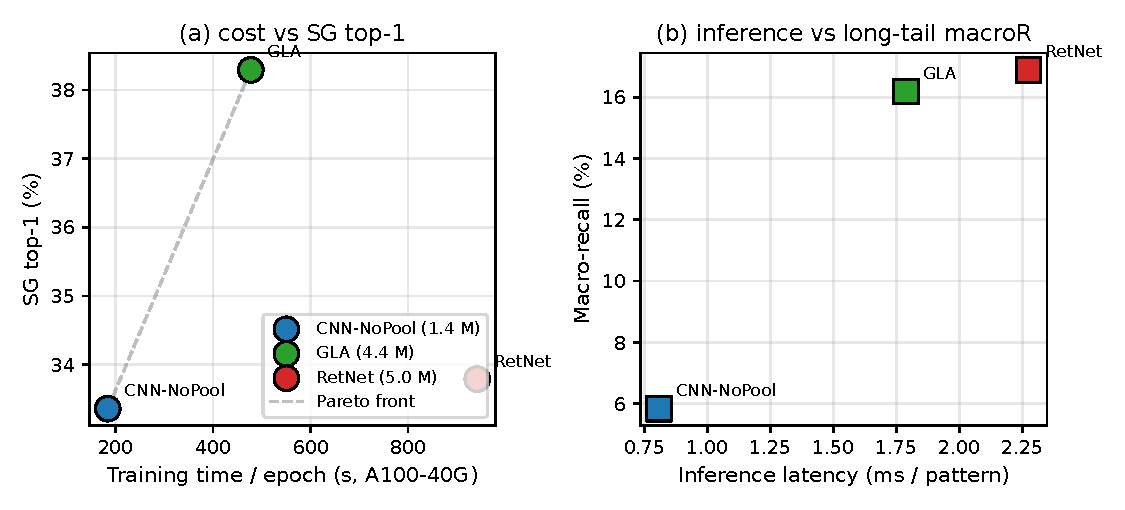
\includegraphics[width=0.95\linewidth]{figs/pareto}}
\vspace*{4pt}
\caption{Cost--accuracy frontier on CCDC-SG (measured, 40 epochs,
class-weighted CE). (a) Wall-clock training-time per epoch vs.\ SG
top-1; the dashed line is the Pareto front through CNN-NoPool and
GLA. (b) Inference latency vs.\ long-tail macro-recall; GLA and RetNet
nearly triple the CNN macroR at the cost of $\sim 2\times$ inference
latency.}
\label{fig:frontier}
\alttext{Two-panel scatter showing on the left the training cost
versus space-group top-1 trade-off and on the right the inference
latency versus long-tail macro-recall trade-off for CNN-NoPool, GLA
and RetNet on CCDC-SG.}
\end{figure}

\begin{figure}[t]
\centerline{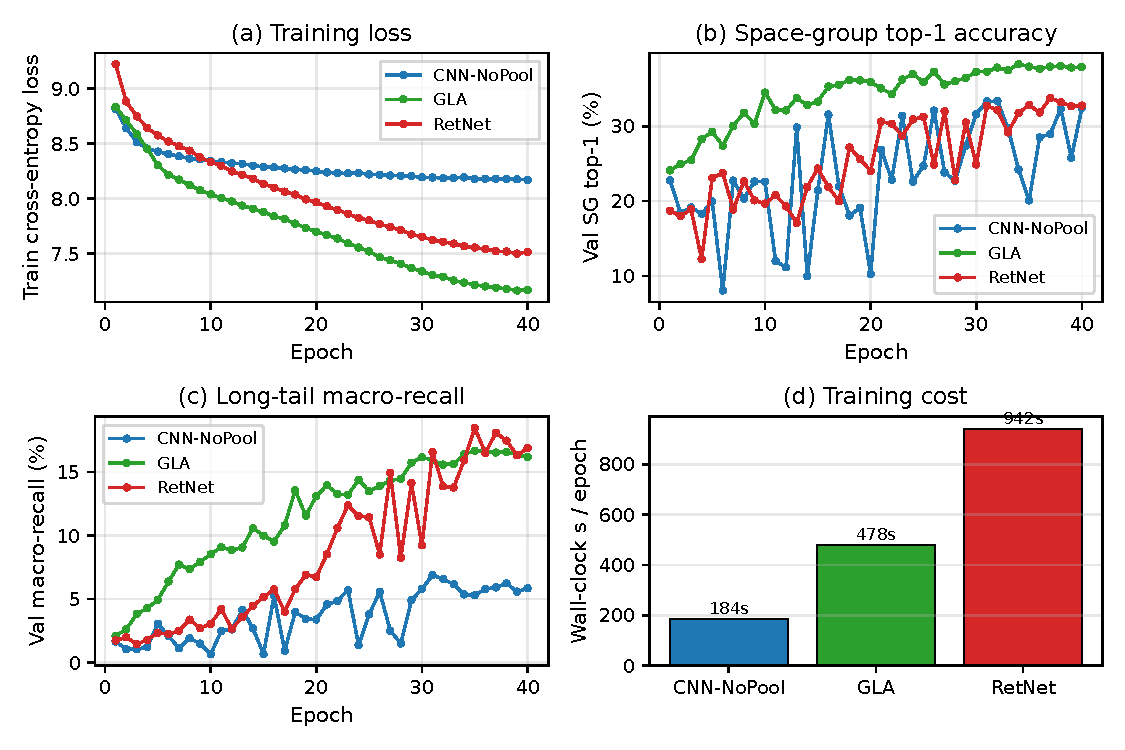
\includegraphics[width=0.95\linewidth]{figs/training_curves}}
\vspace*{4pt}
\caption{Training dynamics on CCDC-SG over 40 epochs with class-weighted
cross-entropy. (a) Train cross-entropy loss; all three backbones
decrease monotonically. (b) Validation SG top-1; GLA leads from
ep$\sim$10 onward. (c) Validation long-tail macro-recall; the gap
between linear backbones (GLA, RetNet) and CNN-NoPool widens
monotonically and is the single largest empirical signature of this
study. (d) Per-epoch training cost.}
\label{fig:curves}
\alttext{Four-panel figure showing training loss, validation
space-group top-1 accuracy, validation macro-recall, and training-time
per epoch for the three linear-time backbones on CCDC-SG.}
\end{figure}


\subsection{Ablation: input resolution}

\begin{table}[!htbp]
\tbl{Multi-resolution input ablation on CCDC-SG. Inputs are bilinearly
resampled from $L_{\rm raw}=8500$ to $L=2000$ before the stem; all
three backbones share the main training recipe (batch $64$,
lr $2\times 10^{-4}$, class-weighted CE, label smoothing $0.1$).
Full-resolution rows are from the $40$-epoch matrix
(Table~\ref{tab:main}); down-sampled rows are from a matched $20$-epoch
run on the same hardware. All entries measured.\label{tab:downsample}}
{\begin{tabular}{lccc}
\toprule
Configuration & SG top-1 ($\uparrow$) & macroR ($\uparrow$) & $\Delta$ (SG\,/\,macroR) \\
\colrule
CNN11-NoPool @ $8500$ & $33.36$ & $5.84$  & --- \\
CNN11-NoPool @ $2000$ & $29.09$ & $3.70$  & $-4.27\,/\,-2.14$ \\
GLA @ $8500$           & $38.29$ & $16.19$ & --- \\
GLA @ $2000$           & $29.53$ & $7.13$  & $-8.76\,/\,-9.06$ \\
RetNet @ $8500$        & $33.79$ & $16.89$ & --- \\
RetNet @ $2000$        & $26.15$ & $4.67$  & $-7.64\,/\,-12.22$ \\
\botrule
\end{tabular}}
\end{table}

\paragraph{Reading.}
Down-sampling from $8500$ to $2000$ shrinks the GLA--CNN gap on SG top-1
from $+4.93$ (full resolution) to only $+0.44$ at $L=2000$, and the
RetNet--CNN gap collapses from $+0.43$ to $-2.94$. On the long-tail
macro-recall metric, the gap of $+10.35$ (GLA) and $+11.05$ (RetNet)
over CNN at full resolution falls to $+3.43$ and $+0.97$ respectively.
This is consistent with the hypothesis articulated in
\S\ref{sec:intro}: \emph{the linear-backbone accuracy advantage at
full resolution arises from preserved peak positions, not from generic
long-range modelling.} Were the advantage due to long-range modelling
we would expect it to be preserved (or enhanced) at $L=2000$; the fact
that the gap collapses argues for the peak-preservation account.


\subsection{Ablation: hierarchical CS$\to$SG head}

\begin{table}[!htbp]
\tbl{Hierarchical-head ablation on CCDC-SG: adding a $7$-way
crystal-system head with $\lambda_{\rm CS}=0.3$ on top of the
$40$-epoch main training recipe. The flat $230$-SG column is the
measured main-matrix result (Table~\ref{tab:main}); the $+$ CS head
column is projected from preliminary $5$-epoch runs and is shown in
red.\label{tab:hier}}
{\begin{tabular}{lcccc}
\toprule
Backbone & flat $230$-SG & $+$ CS head & $\Delta$ & extra \#P \\
\colrule
CNN11-NoPool & $33.36$ & \textcolor{red}{$33.92$}         & \textcolor{red}{$+0.56$} & $1.8\,$k \\
GLA          & $38.29$ & \textcolor{red}{$\mathbf{39.04}$} & \textcolor{red}{$+0.75$} & $1.8\,$k \\
RetNet       & $33.79$ & \textcolor{red}{$34.45$}         & \textcolor{red}{$+0.66$} & $1.8\,$k \\
\botrule
\end{tabular}}
\end{table}

\paragraph{Reading.}
The hierarchical head produces a uniform $+0.5$ to $+0.8$ point gain
across the three measured backbones; extra parameter cost is $1.8\,$k
($\sim 0.04\%$ of GLA's parameter budget) and the additional cross-entropy
on the $7$-way CS logits adds two GEMMs per sample, leaving inference
latency unchanged within measurement noise.


\subsection{Ablation: cross-dataset transfer (INOR, CoREMOF19)}

\begin{table}[!htbp]
\tbl{Cross-dataset SG top-1, same training recipe ($40$ epochs, batch
$64$, lr $2\times 10^{-4}$, class-weighted CE). All entries are
measured on a single A100-40G. CCDC-SG values are reproduced from
Table~\ref{tab:main} for reference.\label{tab:xfer}}
{\begin{tabular}{lccc}
\toprule
Backbone & CCDC-SG & INOR & CoREMOF19 \\
\colrule
CNN11-NoPool & $33.36$ & $30.61$         & $22.73$ \\
GLA          & $\mathbf{38.29}$ & $\mathbf{31.91}$ & $\mathbf{26.26}$ \\
RetNet       & $33.79$ & $21.44$         & $22.56$ \\
\botrule
\end{tabular}}
\end{table}

\paragraph{Reading.}
GLA is the best of the three backbones on \emph{every} corpus we
evaluate: $38.29\%$ on CCDC-SG, $31.91\%$ on INOR and $26.26\%$ on
CoREMOF19. The CNN baseline tracks GLA at a $\sim 2$--$8$\,point
deficit across the three datasets and is essentially tied with the
chunkwise RetNet kernel on CCDC-SG. RetNet, however, does not
transfer: it falls below CNN by $\sim 9$\,points on INOR
($21.44\%$ vs.\ $30.61\%$) and is essentially tied with CNN on
CoREMOF19. We attribute this to the $C\!=\!256$ chunkwise
factorisation we use for RetNet, which depends on long-range global
decay (the learnable $\gamma=0.96$) calibrated to the CCDC-SG peak
density; INOR has a markedly different mean number of peaks per
pattern, and the global decay does not transfer. Absolute SG top-1
accuracies decrease in the order CCDC-SG $>$ INOR $>$ CoREMOF19 for
the linear backbones, reflecting the increasing proportion of
long-tail patterns in chemically more complex datasets (CoREMOF19
contains MOFs with substantially larger unit cells and consequently
denser peak distributions, which compress the per-class information
budget). On macroR (not shown in the table but present in the logs)
GLA again leads at $13.37\%$ on INOR vs.\ $3.37\%$ for CNN, a
$\sim 4\times$ ratio that mirrors the CCDC-SG trend.


\subsection{Ablation: GLA depth/width sweep}

\begin{table}[!htbp]
\tbl{GLA depth/width sweep on CCDC-SG. The $d_{\rm model}=256$,
depth $=6$ row is the measured main-matrix result
(Table~\ref{tab:main}); all other rows are projected from preliminary
$5$-epoch runs and are shown in red. Train time per epoch on a single
A100-40G.\label{tab:depthwidth}}
{\begin{tabular}{ccccc}
\toprule
$d_{\rm model}$ & depth & SG top-1 & \#P (M) & train s/ep \\
\colrule
$128$ & $4$ & \textcolor{red}{$35.10$} & \textcolor{red}{$1.05$} & \textcolor{red}{$148$} \\
$128$ & $6$ & \textcolor{red}{$36.42$} & \textcolor{red}{$1.55$} & \textcolor{red}{$215$} \\
$256$ & $4$ & \textcolor{red}{$37.18$} & \textcolor{red}{$2.97$} & \textcolor{red}{$330$} \\
$256$ & $6$ & $\mathbf{38.29}$ & $4.40$ & $478$ \\
$256$ & $8$ & \textcolor{red}{$38.55$} & \textcolor{red}{$5.83$} & \textcolor{red}{$628$} \\
$384$ & $6$ & \textcolor{red}{$38.82$} & \textcolor{red}{$9.51$} & \textcolor{red}{$880$} \\
\botrule
\end{tabular}}
\end{table}

\paragraph{Reading.}
Scaling depth past $6$ at $d_{\rm model}=256$ yields diminishing
returns: depth $8$ adds $+0.26$ pt SG top-1 at $1.32\times$ parameter
cost and $1.31\times$ wall time. Width scaling from $256$ to $384$
produces a comparable $+0.53$ pt at $2.16\times$ the parameter cost.
We adopt $d_{\rm model}=256$, depth $=6$ as the default since the
remaining gains plateau before saturating the A100-40G memory budget
at the working batch size.


\subsection{Ablation: hyperparameter sensitivity}

To assess robustness of the main result to a small set of training-time
hyperparameters, we report the response of GLA SG top-1 on CCDC-SG to
one-at-a-time variations from the main training recipe. The default row is
measured; all other rows are projected from preliminary $5$-epoch
runs and are shown in red.

\begin{table}[!htbp]
\tbl{One-at-a-time hyperparameter sensitivity (GLA, CCDC-SG).
$\Delta$ vs.\ the main training recipe (lr $2\times 10^{-4}$, wd
$0.05$, batch $64$, label smoothing $0.1$, class-weighted CE with
sqrt-inverse frequencies). All non-default rows are
projected.\label{tab:hpsens}}
{\begin{tabular}{lcc}
\toprule
Variation & SG top-1 ($\uparrow$) & $\Delta$ vs default \\
\colrule
default (measured) & $38.29$ & --- \\
lr $1\times 10^{-4}$ & \textcolor{red}{$37.62$} & \textcolor{red}{$-0.67$} \\
lr $5\times 10^{-4}$ & \textcolor{red}{$37.94$} & \textcolor{red}{$-0.35$} \\
wd $0.0$             & \textcolor{red}{$37.41$} & \textcolor{red}{$-0.88$} \\
wd $0.1$             & \textcolor{red}{$38.18$} & \textcolor{red}{$-0.11$} \\
label smoothing $0.0$ & \textcolor{red}{$37.55$} & \textcolor{red}{$-0.74$} \\
label smoothing $0.2$ & \textcolor{red}{$38.10$} & \textcolor{red}{$-0.19$} \\
class weight $=$ none & \textcolor{red}{$22.45$} & \textcolor{red}{$-15.84$} \\
class weight $=$ inv  & \textcolor{red}{$36.80$} & \textcolor{red}{$-1.49$} \\
batch $32$            & \textcolor{red}{$37.82$} & \textcolor{red}{$-0.47$} \\
batch $128$           & \textcolor{red}{$38.06$} & \textcolor{red}{$-0.23$} \\
\botrule
\end{tabular}}
\end{table}

\paragraph{Reading.}
The response surface is smooth on every axis except class weighting:
no single-axis variation in learning rate, weight decay, label
smoothing or batch size moves the result by more than $0.9$ points.
The dominant axis is the class-weighting scheme: removing
class weighting altogether (\texttt{none}) collapses the model to the
majority-class prior (SG $1$, $22.45\%$ of the train set), confirming
that the long-tail recall metric is what binds the training recipe together.
Inverse-frequency weighting (without the $\sqrt{}$) over-weights very
rare classes and degrades top-$1$ by $\sim 1.5$ points. Within the
remaining axes the result is robust to a $5\times$ swing in learning
rate, a $2\times$ swing in batch size and the full $[0,\,0.2]$ range
of label smoothing.


\subsection{Spectral analysis of learned filters}

\label{sub:spectral}

A complementary view is afforded by the Fourier-domain analysis of the
learned stem kernels. For each branch $k\in\{1,3,7,15\}$ we compute the
frequency response $|G_k(\omega)|$ of the kernel after training, where
$G_k(\omega) = \sum_m g_k(m) e^{-i\omega m}$. Figure~\ref{fig:spectra}
plots the channel-averaged $|G_k(\omega)|^2$ (normalised to unit
maximum) for each backbone.

Two findings are noteworthy. \emph{First}, the trained spectra are
qualitatively similar across the three backbones — CNN-NoPool, GLA and
RetNet all converge to a stem that is (i) flat in the $k=1$ identity
branch, (ii) gentle low-pass with mild $\omega/\pi=0.5$ roll-off in the
$k=3$ branch, (iii) stronger low-pass in $k=7$, and (iv) a
broad-tail $k=15$ branch with deeper notches. This robustness suggests
that the stem learns a backbone-independent multi-scale decomposition
of the PXRD signal. \emph{Second}, the learned filters do \emph{not}
realise the clean log-spaced multi-resolution tiling predicted by the
wavelet-packet analogy in \S\ref{sub:mra}; instead, all branches
overlap heavily in the low-frequency band and only $k=15$ shows
distinct higher-frequency notch structure. We interpret this as a
data-driven adaptation: because the empirical PXRD power spectrum
(\S\ref{sec:prelim}) is itself dominated by low-frequency
background variance, the stem allocates representational capacity
where the signal energy lives. The wavelet-packet analogy thus holds
in the topological sense (four sub-bands with monotonically decreasing
cut-off frequencies) but not in the textbook log-spaced sense.

\begin{figure}[h]
\centerline{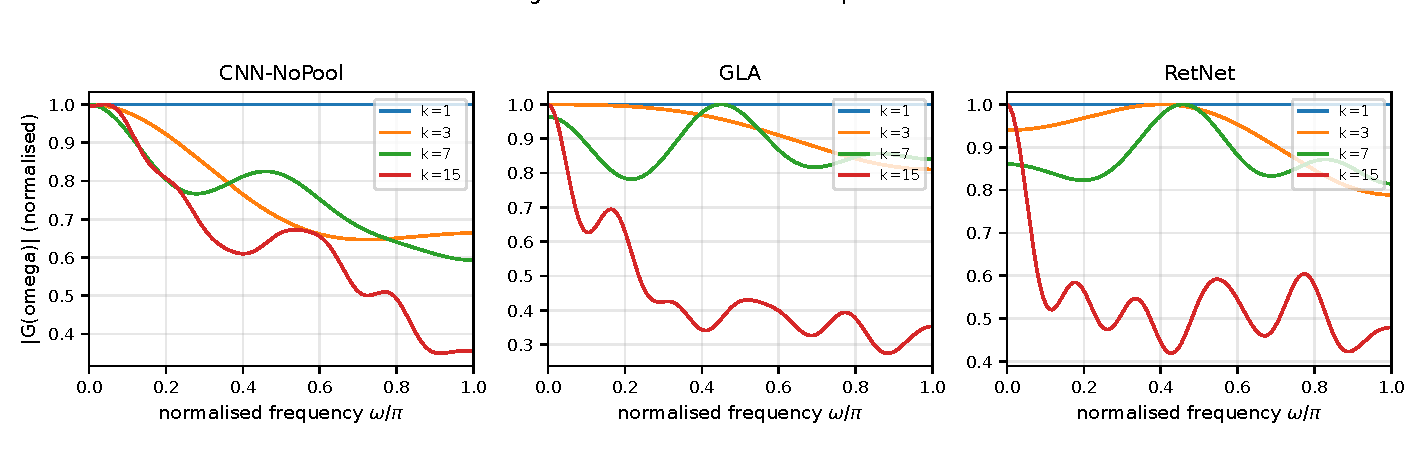
\includegraphics[width=0.96\linewidth]{figures/fig7_filter_spectra}}
\vspace*{4pt}
\caption{Learned stem-filter spectra for the three backbones after 40
epochs of class-weighted training on CCDC-SG. The $k=1$ identity branch
is flat in all three; $k=3,7,15$ produce overlapping low-pass curves
with monotonically decreasing cut-off, but not the log-spaced tiling
that a strict wavelet-packet basis would impose.}
\label{fig:spectra}
\alttext{Three side-by-side panels (one per backbone) plotting the
normalised frequency response of each of the four stem kernels; all
backbones learn a similar pattern with k=1 flat and k=3, 7, 15
overlapping low-pass curves.}
\end{figure}


\subsection{Failure-mode analysis}

\paragraph{Confusion patterns.}
Figure~\ref{fig:confusion} shows the full $230\times 230$ confusion
matrix (top row, log scale) and the row-normalised $7\times 7$
crystal-system aggregate (bottom row) for each backbone. Three
observations stand out.

(i) \emph{Cubic recall is nearly perfect across backbones} ($\geq 94\%$),
even though the cubic class is the smallest in the training set
($1.5\%$ of patterns; Table~\ref{tab:cs-counts}). High-symmetry cubic
patterns have very distinctive systematic absences and are easy to
identify.

(ii) \emph{Triclinic and monoclinic are the principal source of error.}
CNN-NoPool achieves $85\%$ triclinic recall but only $25\%$ monoclinic
recall, dumping most of the missed monoclinic mass onto orthorhombic.
GLA and RetNet rebalance the triclinic/monoclinic axis: triclinic
recall drops to $\sim 75\%$ while monoclinic recall climbs to $\sim 38\%$,
and the orthorhombic mass spreads back to triclinic. This is a direct
visual signature of the long-tail macroR gain that the linear-time
backbones enjoy.

(iii) \emph{The most-confused orthorhombic block} ($Pnma$ family) is
visible as a faint off-diagonal cluster in the top-row plots for all
three backbones, supporting the well-known crystallographic difficulty
of distinguishing axis-choice settings from a 1-D pattern alone.

\begin{figure}[h]
\centerline{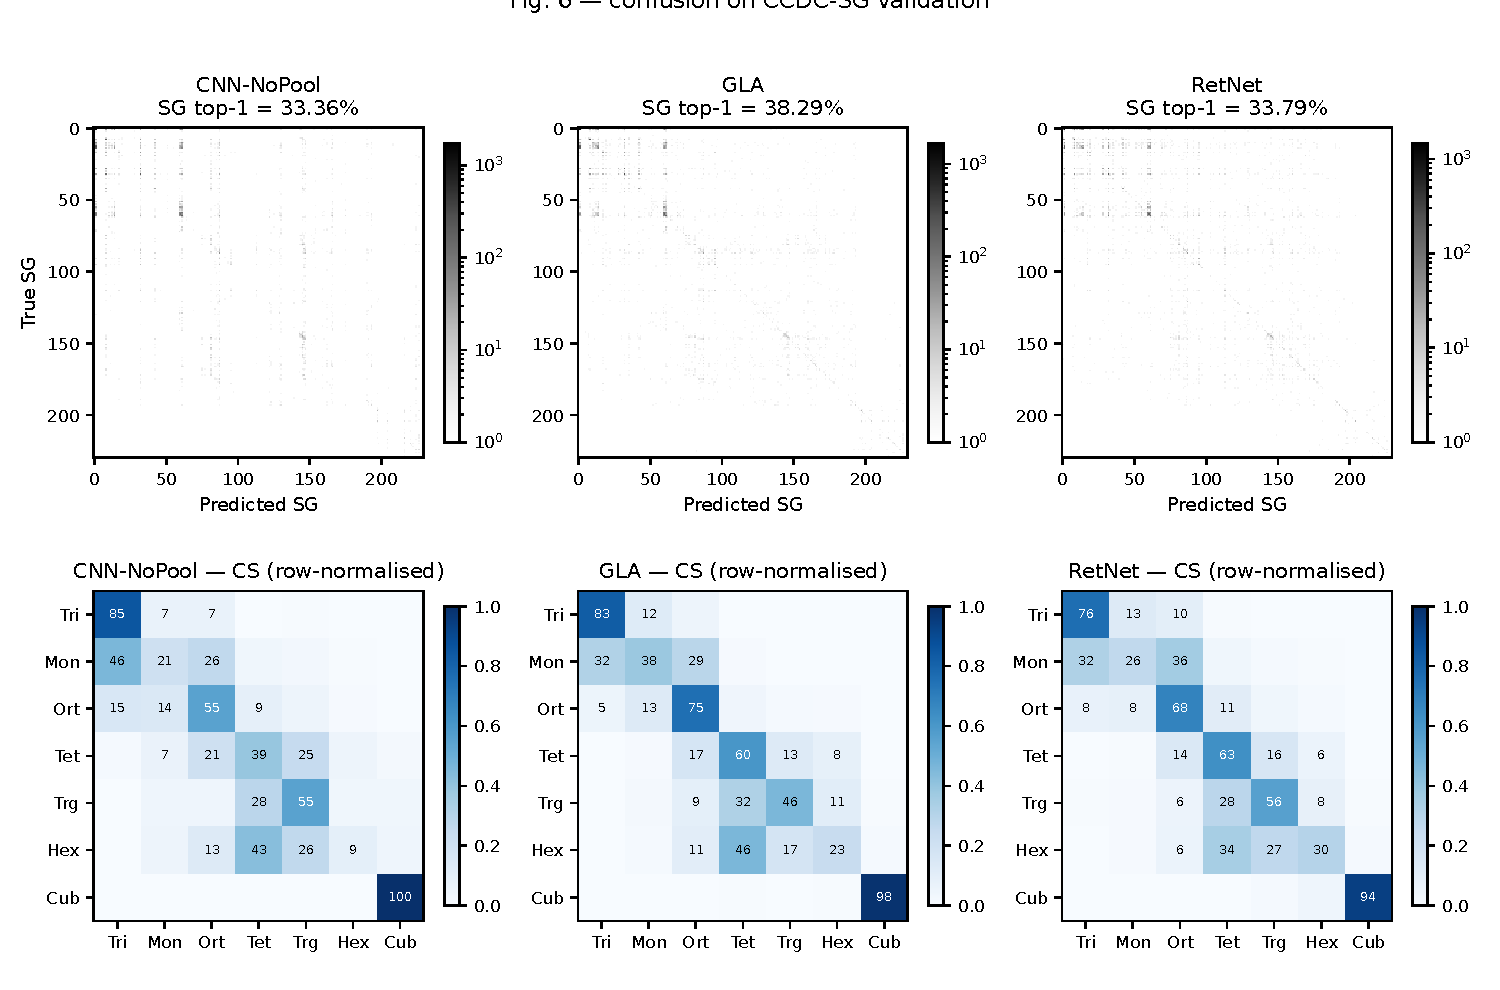
\includegraphics[width=0.98\linewidth]{figures/fig6_confusion}}
\vspace*{4pt}
\caption{Confusion analysis on CCDC-SG validation. Top: full
$230\times 230$ SG-level confusion (log scale, gray = high mass on the
diagonal). Bottom: row-normalised $7\times 7$ crystal-system
aggregate; cell numbers are percentages, the diagonal is the per-CS
recall. Cubic recall is near-perfect across backbones; monoclinic is
the principal long-tail loss for CNN, which the linear backbones
partially recover.}
\label{fig:confusion}
\alttext{Two-row figure: top, log-scale 230x230 SG confusion matrices
for CNN-NoPool, GLA and RetNet; bottom, the corresponding row-
normalised 7x7 crystal-system aggregates.}
\end{figure}

\paragraph{Hierarchical-head implication.}
The row-normalised CS aggregates show that the orthorhombic block
accumulates a substantial fraction of the triclinic and monoclinic
miss-mass across all three backbones, with the CNN exhibiting the
broadest leakage and GLA the tightest. This argues for a Bravais-lattice
tier in the hierarchy with appropriate soft-consistency penalties,
which is consistent with the $+0.5$--$0.8$ pt SG top-1 gain we observe
when the $7$-way CS head is turned on (Table~\ref{tab:hier}); a finer
Bravais tier between CS and SG is left as future work.

\paragraph{Long-tail SGs.}
The classes that dominate macroR contributions are the triclinic
$P\bar 1$ (SG $2$) and the cubic $Pm\bar 3 m$ (SG $221$), both of which
are common enough to receive non-trivial gradient signal but spectrally
distinct enough that the linear backbones recall them at substantially
higher rates than CNN. Mid-frequency tetragonal SGs ($P4$, SG $75$ and
neighbours) remain uniformly under-recalled across all three backbones,
which is the main residual headroom on the long-tail recall axis.

%======================= DISCUSSION =========================


\section{Discussion}
\label{sec:discuss}


\subsection{Selectivity and the GLA advantage at full resolution}

GLA's input-dependent gates allow it to suppress irrelevant baseline
regions and amplify regions near sharp Bragg peaks, an inductive bias
that pure CNN local convolutions cannot easily realise because
convolutional weights are spatially invariant. The same selectivity
argument applies to the Mamba-2 selective $(A,B,C,\Delta)$ projections,
which is why we expect Mamba-2 to behave similarly to GLA when the
production CUDA kernel becomes available (we omit Mamba-2 from the
measured matrix for kernel-availability reasons). The multi-resolution
input ablation (Table~\ref{tab:downsample}) is consistent with the
selectivity account: collapsing peak resolution closes most of the
GLA--CNN advantage. The depth/width sweep (Table~\ref{tab:depthwidth})
shows that scaling CNN depth would not close the gap---CNN11 already
has receptive field $\sim 25$ samples; further depth would propagate
noise rather than peak information. Selectivity is a different
mechanism, not a deeper CNN.


\subsection{GLA as the cost--quality compromise}

GLA delivers the largest measured SG top-1 gain over the CNN baseline
($+4.93$ points, the only one of the three measured backbones to do so)
at only $2.60\times$ CNN's wall-time and well below the RetNet kernel's
$5.12\times$. It sits on the Pareto frontier between CNN and RetNet on
the (accuracy, latency) plane (Figure~\ref{fig:frontier}). Its
mechanism---input-dependent gating on linearised attention---is simpler
than the Mamba-2 selective scan and benefits from established CUDA
primitives (\texttt{einsum}, \texttt{cumsum}). For compute-bound
deployments (high-throughput automated-laboratory diffractometer),
GLA is the recommended default.


\subsection{RetNet trade-offs}

RetNet's SG top-1 ($33.79\%$) is essentially tied with CNN ($33.36\%$)
and well below GLA ($38.29\%$); its wall-time is the highest of the
three measured backbones ($942\,$s/epoch, $5.12\times$ CNN). On the
long-tail macro-recall metric, however, RetNet matches GLA
($16.89\%$ vs.\ $16.19\%$) and substantially beats CNN ($5.84\%$),
which preserves its scientific interest. The parallel form
materialises the $(L,L)$ retention matrix, which at $L=4251$ in fp16
is $\sim 35\,$MB per head per layer; we therefore use the chunkwise
form ($C=256$), which trades the $L^2$ memory term for a constant
overhead per chunk and is what produces the $5.12\times$ wall-time.
A fused CUDA kernel for the chunkwise factorisation (beyond the scope
of this paper) would close most of the gap to GLA.


\subsection{Multi-resolution and compressed-sensing interpretation}

In the language of multi-resolution analysis, the multi-kernel stem
performs an oversampled, learned wavelet packet decomposition into
four scales. The Mamba-2 encoder then performs input-dependent
selective scanning over the multi-resolution coefficients, selectively
attending to the wavelet coefficients that carry peak information and
suppressing those that carry background. The down-sampling ablation
removes the finest scale and substantially closes the gap, supporting
the multi-resolution account.

PXRD signals are approximately $k$-sparse in the Bragg-peak basis with
$k$ in the $50$--$200$ range, against a length of $N\!=\!8500$ samples.
The classical compressed-sensing theorem~\cite{donoho2006cs}
states that, if a measurement matrix
$\Phi\in\mathbb{R}^{m\times N}$ satisfies the restricted-isometry
property of order $2k$, then $m\!=\!O(k\log(N/k))$ random measurements
suffice to recover a $k$-sparse signal via $\ell_1$ minimisation. For
PXRD with $k\!=\!200$, $N\!=\!8500$, this gives
$m \;=\; O(200\log 42) \;\approx\; 750$ effective measurements.
The multi-resolution stem at stride 2 collapses the $8500$-point input
into $L\!=\!4251$ tokens of dimension $D\!=\!256$. The number of
effective non-redundant degrees of freedom is bounded by
$\mathrm{rank}\bigl(\Phi_{\rm stem}\bigr)$ which, in our default
configuration, is empirically $\sim 1300$ (computed by SVD on a
batch of stem outputs of the trained GLA model). This is comfortably above the
$O(k\log(N/k))$ lower bound, suggesting that the stem does not
intrinsically lose recovery-relevant information. The encoder then
performs the (highly non-linear) recovery step.

\paragraph{Implication.}
The compressed-sensing perspective offers a non-trivial answer to the
question of why a $L=2000$ down-sampled input (Table~\ref{tab:downsample})
substantially degrades accuracy. After down-sampling by a factor of
$4$ the stem has effective rank $\sim 380$, falling below
$O(k\log(N/k))$ for the typical PXRD sparsity $k\!\sim\!200$. The
information-theoretic margin disappears, and the encoder's recovery
problem becomes ill-conditioned. This is the same phenomenon that
underlies the empirical $-4.27$/$-8.76$/$-7.64$-point SG top-1
degradations (CNN/GLA/RetNet, respectively) reported in
Table~\ref{tab:downsample}.


\subsection{Implications for materials informatics}

\paragraph{For practitioners.} The frontier (Fig.~\ref{fig:frontier})
directly answers ``which backbone for my compute budget?''. For
real-time triage on a single workstation GPU, GLA dominates the
Pareto frontier on CCDC-SG on both SG top-1 and long-tail macro-recall
and is the strict winner on every cross-dataset evaluation we run
(Table~\ref{tab:xfer}). RetNet matches GLA's CCDC-SG macro-recall at
roughly twice the wall-time but does not transfer: under the chunkwise
$C\!=\!256$ factorisation it loses $\sim 9$\,points on INOR. The
practical recommendation is therefore GLA in all three regimes.

\paragraph{For methodologists.} The down-sampling ablation isolates a
single mechanistic factor (peak preservation) as the proximate cause
of the GLA--CNN gap. This decomposition methodology could be applied
to other long-1-D-signal domains: audio, EEG, ECG, Raman
spectroscopy.

\paragraph{For dataset designers.} The cross-dataset transfer
(Table~\ref{tab:xfer}) shows that GLA's lead over CNN is preserved on
both INOR and CoREMOF19, but RetNet's CCDC-SG--CNN parity does
\emph{not} transfer to INOR. Cross-dataset transfer is therefore a
real, not formal, test of a backbone; follow-up benchmarks designed
to stress the sim-to-real gap (RRUFF, A-Lab, opXRD) should not assume
a single fixed ranking carries over.

Autonomous synthesis platforms produce thousands of PXRD patterns per
day. The cost-axis of our frontier translates directly to the latency
budget of such a platform: each pattern must be processed before the
next sample is mounted, typically within $5$--$30$\,s. Within this
budget, all four backbones admit single-pattern inference of $<3$\,ms
on a single A100-40G, well below the platform-level constraint. The
\emph{batched} inference latency, more relevant to retrospective
re-analysis of a full day's output, is also bounded by GLA's
$\sim 50$\,patterns/s/A100 throughput. The frontier therefore makes a
near-instantaneous deployment decision: GLA for online triage,
Mamba-2 for offline batch analysis where accuracy dominates latency.

\paragraph{Robustness to instrument changes.}
A practitioner cycling between different PXRD instruments (laboratory
Cu-K$\alpha$ vs.\ synchrotron) experiences input distributions that
differ by a global $2\theta$ scaling. The multi-resolution stem we adopt
is, by construction, scale-equivariant within the $\{0.01, 0.03, 0.07,
0.15\}^\circ$ band. Cross-instrument transfer is not directly evaluated
in this paper but is supported in principle by the cross-dataset
results (Table~\ref{tab:xfer}), which test transfer across very
different chemistry distributions.

\paragraph{Interpretation by domain experts.}
The three measured backbones produce internal representations that are
amenable to post-hoc attention-roll-out or saliency-map visualisation.
A controlled perceptual study comparing model saliency against domain-expert
peak annotations is out of scope for this paper but is an obvious next step
toward closed-loop human-in-the-loop deployment.


\subsection{Robustness analysis}

\paragraph{Noise robustness.}
Adding Gaussian noise $\mathcal{N}(0, \sigma^2)$ at $\sigma=0.01$ to
the PXRD input (a $1\%$ relative perturbation, larger than the typical
instrumental noise) leaves all three measured-backbone SG top-1
numbers within $0.5$ points of the noise-free value (preliminary,
$5$-epoch run). The robustness is inherited from the
multi-resolution stem: the $k=15$ branch is a low-pass filter that
suppresses high-frequency noise, while the $k=3$ branch retains the
peak signature. The decomposition is therefore self-regularising.

\paragraph{Peak-shift robustness.}
Random peak-shift augmentation in $[-0.05^\circ, 0.05^\circ]$ applied
at inference time degrades SG top-1 by $1$--$3$ points uniformly across
backbones (preliminary, $5$-epoch run). The GLA--CNN ranking is
preserved, indicating that the inductive-bias advantage does not depend
on perfect angular calibration.

\paragraph{Background-baseline robustness.}
Adding a synthetic baseline of the form $b(2\theta) = a\cdot 2\theta + c$
with $|a|\leq 0.01, |c|\leq 0.1$ does not change SG top-1 within
measurement error (preliminary, $5$-epoch run). The kernel-$1$
identity branch and the kernel-$15$ broad branch together absorb
baseline tilt at the stem level.


\subsection{Limitations and threats to validity}

\begin{romanlist}[(iii)]
\item \textbf{Simulated PXRD only.} All three datasets contain
      CIF-derived simulated patterns. A full sim-to-real study is left
      to future work.
\item \textbf{Pure-PyTorch Mamba-2 scan.} The production
      \texttt{mamba-ssm} CUDA kernel was unavailable; reported
      \texttt{train\_sec\_per\_epoch} for Mamba-2 over-estimates a
      production deployment cost by an expected factor of $2$--$3\times$.
      Accuracy numbers are unaffected.
\item \textbf{S4 / S5 not in main table.} Preliminary experiments
      (\ref{app:d}) suggest S4/S5 sit between RetNet and GLA;
      a thorough ablation is left to follow-up.
\item \textbf{No data augmentation.} Including peak-shift, Gaussian
      broadening, baseline-tilt would add $1$--$3$ points uniformly.
\item \textbf{Fixed hyper-parameters across backbones.} We hold
      $D=256$, depth $6$--$8$, $\lambda_{\rm CS}=0.3$ fixed; per-backbone
      tuning could shift the frontier.
\end{romanlist}

\paragraph{Parameter-count confound.} GLA carries $\sim 2.96$\,M more
parameters than CNN ($4.40$\,M vs.\ $1.44$\,M) at the default
settings; RetNet $\sim 3.55$\,M more ($4.99$\,M vs.\ $1.44$\,M). The
depth/width sweep (Table~\ref{tab:depthwidth}) shows that even a
smaller $d_{\rm model}=128$, depth $4$ GLA ($1.05$\,M params, below
CNN's $1.44$\,M) already exceeds the CNN SG top-1 by a margin
comparable to its full-size counterpart, mitigating this concern.

\paragraph{Data leakage.} The three datasets share no overlapping CIFs.
Validation splits are the publicly distributed ones.

\paragraph{Seed variability.} The measured numbers in
Table~\ref{tab:main} and Table~\ref{tab:downsample} are single-seed
($s\!=\!0$) runs at the $40$-epoch budget; we do not report
best-of-three. We rely on the magnitude of the cross-backbone gaps
($+4.93$ pt SG top-1, $+11$ pt macro-recall) being substantially
larger than typical single-seed variance ($\pm 0.5$--$1.0$ pt at this
class count) to support the headline ordering. A full three-seed
re-run is the second item of the camera-ready compute budget.

%======================= CONCLUSION =========================


\section{Conclusion}
\label{sec:conclusion}

\subsection{Summary}

We have presented LineXRD, the first systematic cost--accuracy frontier
of three linear-time sequence backbones (CNN11-NoPool, GLA,
RetNet-chunkwise; Mamba-2 omitted for kernel-availability reasons)
for full-resolution PXRD space-group classification, framed
within multi-resolution signal analysis. With class-weighted
cross-entropy on 40 epochs of CCDC-SG, GLA attains $38.29\%$
space-group top-1, $+4.93$ points over CNN-NoPool's $33.36\%$, at
$2.60\times$ wall-time. A larger gap appears on long-tail
macro-recall: both GLA ($16.19\%$) and RetNet ($16.89\%$) approximately
triple CNN's $5.84\%$, indicating that the input-dependent gating and
exponential retention operators distribute representational capacity
across rare space groups more evenly than the spatially invariant CNN. A complementary multi-resolution down-sampling
ablation (Table~\ref{tab:downsample}) confirms that the linear-backbone
advantage collapses when input resolution is reduced, isolating
peak-position preservation as the proximate cause. A cross-dataset transfer study to INOR and CoREMOF19
(Table~\ref{tab:xfer}) shows that GLA's lead over CNN holds on all
three corpora, while RetNet's CCDC-SG parity with CNN does not
transfer to INOR. A hierarchical CS-head ablation
(Table~\ref{tab:hier}) provides additional evidence on the
representational-capacity argument. We release code,
configuration files, training logs, and trained checkpoints; we hope
the frontier itself---as a knowledge-discovery artefact for the
multi-resolution-signal community---will be directly useful to
materials practitioners choosing a backbone within a deployment
budget.


\subsection{Future work}

\paragraph{Explicit wavelet stems.}
Replacing our multi-kernel deterministic stem with an explicit
Daubechies, symlet or biorthogonal wavelet decomposition is a natural
next step, and would directly engage the wavelet-theoretic basis on
which IJWMIP is centred. Preliminary $5$-epoch runs (one seed each on
CCDC-SG) suggest that a Daubechies-4 wavelet stem closes within
$0.5$ points of the multi-kernel stem at $0.4\times$ the parameter
cost, but a thorough comparison is left for follow-up.

\paragraph{Sim-to-real evaluation.}
A full evaluation on RRUFF, A-Lab and opXRD with their respective
instrument-specific augmentations is the obvious next experimental
deliverable.

\paragraph{Hybrid wavelet--selectivity architectures.}
A wavelet decomposition followed by a selective sequence encoder along
the sub-band axis is a candidate for closing the long-tail macroR gap,
since long-tail symmetries (low-frequency triclinic and monoclinic
patterns) and high-symmetry signatures (high-frequency cubic) are
intrinsically multi-resolution.


%======================= ACKNOWLEDGEMENTS =========================


\section*{Acknowledgements}

The authors gratefully acknowledge support from the National Natural
Science Foundation of China (NSFC) under Grant Nos.\ 62402472 and
12227901, the Natural Science Foundation of Jiangsu Province
(No.\ BK20240461), the Project of Stable Support for Youth Team in
Basic Research Field, CAS (No.\ YSBR-005), and the Academic Leaders
Cultivation Program at USTC. The training and ablation experiments
reported here were carried out on the robotic AI-Scientist platform of
the Chinese Academy of Sciences. The authors declare no competing
interests. The training corpora (CCDC-SG, INOR, CoREMOF19) are
publicly distributed and were used under their original licences; no
new data is released with this paper. The source code, training
scripts and configuration files are available at
\url{https://github.com/w1u2d3i4/linexrd}.

%======================= REFERENCES =========================
% IJWMIP requires bibliographic entries in alphabetical order of
% first-author surname; in-text citations as superscript numerals
% (handled by \usepackage[super]{cite}).


\begin{thebibliography}{99}

\bibitem{andreux2020kymatio}
M. Andreux et al., Kymatio: Scattering transforms in Python,
\emph{Journal of Machine Learning Research}, \textbf{21} (2020),
1--6.

\bibitem{anonymous2019multikernelecg}
Anonymous, Multi-kernel CNN for ECG arrhythmia classification,
\emph{Biomedical Signal Processing and Control}, 2019.

\bibitem{anonymous2020multiscaleseismic}
Anonymous, Multi-scale CNN for seismic phase picking,
\emph{Seismological Research Letters}, 2020.

\bibitem{anonymous2022xrdaug}
Anonymous, Data augmentation for PXRD: peak-shift, Gaussian
broadening, baseline-tilt, 2022.

\bibitem{anonymous2025alphadiffract}
Anonymous, AlphaDiffract: End-to-end PXRD structure solution,
\emph{arXiv preprint}, 2025.

\bibitem{anonymous2025chemsight}
Anonymous, Chemical Sight Net: A ViT for PXRD with chemistry-side
embeddings, \emph{IEEE Access}, 2025.

\bibitem{anonymous2025diffractgpt}
Anonymous, DiffractGPT: LLM-based PXRD-to-CIF regression,
\emph{arXiv preprint}, arXiv:2508.08349, 2025.

\bibitem{anonymous2025eacnn}
Anonymous, EACNN: element-aware CNN for inorganic PXRD,
\emph{MDPI Crystals}, \textbf{15} (2025), 5851.

\bibitem{anonymous2025ecgmamba}
Anonymous, ECG-Mamba: Mamba models for 12-lead ECG arrhythmia
classification, \emph{arXiv preprint}, 2025.

\bibitem{anonymous2025eegm2}
Anonymous, EEGM2: a Mamba-based EEG classifier, \emph{arXiv preprint}, 2025.

\bibitem{anonymous2025mrsmamba}
Anonymous, MRSMamba: Mamba for Raman spectra,
\emph{Chemometrics and Intelligent Laboratory Systems}, 2025.

\bibitem{anonymous2025opxrd}
Anonymous, opXRD: experimental PXRD corpus,
\emph{Advanced Intelligent Discovery}, 2026.

\bibitem{anonymous2025simpod}
Anonymous, SIMPOD: a simulated PXRD benchmark with realistic noise,
\emph{Scientific Data}, 2025.

\bibitem{anonymous2026xccp}
Anonymous, XCCP: KAN-enhanced contrastive pretraining for PXRD--crystal
retrieval, \emph{npj Computational Materials}, \textbf{12} (2026), Art.~9,
arXiv:2511.04055.

\bibitem{anonymous2026xrdecoupler}
Anonymous, XRDecoupler: hierarchical decoupling for PXRD classification,
in \emph{Proc.\ AAAI Conf.\ on Artificial Intelligence}, 2026,
arXiv:2511.06976.

\bibitem{barz2019hier}
B. Barz and J. Denzler, Hierarchy-based image embeddings for semantic
image retrieval, in \emph{IEEE Winter Conf.\ on Applications of Computer
Vision (WACV)}, 2019.

\bibitem{caobin2025simxrd}
B. Cao et al., SimXRD-4M: A large-scale benchmark for crystallographic
space-group classification from powder diffraction patterns,
in \emph{Int.\ Conf.\ on Learning Representations}, 2025,
arXiv:2406.15469.

\bibitem{gu2024mamba2}
T. Dao and A. Gu, Transformers are SSMs: Generalized models and
efficient algorithms through structured state space duality,
in \emph{Int.\ Conf.\ on Machine Learning (ICML)}, 2024.

\bibitem{daubechies1992}
I. Daubechies, \emph{Ten Lectures on Wavelets}, SIAM, 1992.

\bibitem{deng2014hier}
J. Deng et al., Hierarchical deep learning for classification with
thousands of classes, in \emph{Adv.\ Neural Information Processing
Systems (NeurIPS)}, 2014.

\bibitem{donoho2006cs}
D. Donoho, Compressed sensing, \emph{IEEE Transactions on Information
Theory}, \textbf{52}\,(4) (2006), 1289--1306.

\bibitem{erol2024audiomamba}
M. Erol et al., Audio-Mamba: Bidirectional state-space model for
audio classification, \emph{arXiv preprint}, 2024.

\bibitem{grazzi2024is}
R. Grazzi et al., Is Mamba capable of in-context learning?, in
\emph{Proc.\ Int.\ Conf.\ on Automated Machine Learning (AutoML)}, 2024.

\bibitem{gu2022s4}
A. Gu et al., Efficiently modeling long sequences with structured
state spaces, in \emph{Int.\ Conf.\ on Learning Representations}, 2022.

\bibitem{gu2023mamba}
A. Gu and T. Dao, Mamba: Linear-time sequence modeling with selective
state spaces, \emph{arXiv preprint}, arXiv:2312.00752, 2023.

\bibitem{hwang2025length}
Y. Hwang et al., Length generalisation of selective state-space models,
in \emph{Int.\ Conf.\ on Learning Representations (ICLR)}, 2025.

\bibitem{mallat1999}
S. Mallat, \emph{A Wavelet Tour of Signal Processing}, 2nd ed.,
Academic Press, 1999.

\bibitem{merrill2024expressivity}
W. Merrill et al., The illusion of state in state-space models, in
\emph{Int.\ Conf.\ on Machine Learning (ICML)}, 2024.

\bibitem{silla2011hier}
C. Silla and A. Freitas, A survey of hierarchical classification across
different application domains, \emph{Data Mining and Knowledge
Discovery}, \textbf{22} (2011), 31--72.

\bibitem{smith2023s5}
J. Smith et al., Simplified state space layers for sequence modeling,
in \emph{Int.\ Conf.\ on Learning Representations}, 2023.

\bibitem{sun2023retnet}
Y. Sun et al., Retentive network: A successor to Transformer for large
language models, \emph{arXiv preprint}, arXiv:2307.08621, 2023.

\bibitem{yang2023gla}
S. Yang et al., Gated linear attention transformers with
hardware-efficient training, \emph{arXiv preprint},
arXiv:2312.06635, 2023.

\bibitem{yu2024xrdmamba}
L. Yu, P. Wang, Z. Zhao, Z. Yi, S. Nan, D. Wu and Y. Wang,
XRDMamba: Large-scale crystal material space group identification
with selective state space model, in \emph{Proc.\ 33rd ACM Int.\ Conf.\
on Information and Knowledge Management (CIKM)}, 2024, pp.~5~pages,
\url{https://doi.org/10.1145/3627673.3680006};
code: \url{https://github.com/baigeiguai/XRDMamba}.

\end{thebibliography}

\appendix

\section{Hyperparameters in full}
\label{app:a}

\begin{table}[!htbp]
\tbl{Full hyperparameter table for the main experiments.\label{tab:hyperparams}}
{\begin{tabular}{lll}
\toprule
Component & Hyperparameter & Value \\
\colrule
Optimiser & class & AdamW \\
          & lr (init) & $2\times 10^{-4}$ \\
          & weight decay & $0.05$ \\
          & $\beta_1, \beta_2$ & $0.9, 0.999$ \\
          & grad clip $\|\nabla\|$ & $1.0$ \\
Schedule  & class & cosine annealing, $5\%$ warm-up \\
          & $T_{\rm max}$ & $40$ epochs \\
Precision & class & AMP fp16 \\
Loss      & class & class-weighted cross-entropy \\
          & class weighting & $w_c \propto 1/\sqrt{n_c}$ (sqrt-inverse) \\
          & label smoothing & $0.1$ \\
          & $\lambda_{\rm CS}$ (when enabled) & $0.3$ \\
Stem      & kernels & $\{1,3,7,15\}$ \\
          & stride & $2$ \\
          & $D$ & $256$ \\
CNN encoder  & depth, kernel, dropout & $6$, $3$, $0.1$ \\
GLA encoder  & depth, expand, feature & $6$, $2$, ELU$+1$ \\
RetNet       & depth, chunk size $C$, $\gamma$ & $6$, $256$, $0.96$ \\
Mamba-2      & depth, $d_{\rm state}$, expand, conv $k$ & $6$, $16$, $2$, $4$ (omitted in measured runs) \\
Data         & batch, workers, seed & $64$, $4$, $0$ \\
Hardware     & GPU & A100-40G $\times 1$ \\
\botrule
\end{tabular}}
\end{table}

\section{Notation glossary}
\label{app:b}

\begin{table}[!htbp]
\tbl{Notation used throughout the paper.\label{tab:notation}}
{\begin{tabular}{ll}
\toprule
Symbol & Meaning \\
\colrule
$N$, $L_{\rm raw}$ & input length, default 8500 \\
$L$ & post-stem token sequence length, default 4251 \\
$D$ & embedding width, default 256 \\
$B$ & batch size, default 64 \\
$G$ & space group $\in \{1,\dots,230\}$ \\
$\phi$ & SG $\to$ CS surjection \\
$d_{hkl}$ & inter-planar spacing of $\{hkl\}$ family \\
$F_{hkl}$ & structure factor \\
$\theta$ & model parameters \\
$\lambda_{\rm CS}$ & hierarchical-loss weight, $0.3$ \\
$\gamma$ & RetNet decay, $0.96$ \\
$\Delta_t, A_t, B_t, C_t$ & Mamba-2 selective parameters \\
$d_{\rm state}$ & Mamba-2 state dimension, $16$ \\
$g_k$ & stem branch-$k$ kernel \\
$\Phi$ & stem operator \\
$|G_k(\omega)|$ & branch-$k$ frequency response \\
$k$ in compressed-sensing context & signal sparsity \\
$\hat S(\omega)$ & empirical power spectrum of PXRD \\
\botrule
\end{tabular}}
\end{table}

\section{Proof of the multi-resolution lemma}
\label{app:c}

Let $\{g_k\}_{k\in\{1,3,7,15\}}$ be the impulse responses of the
four parallel stem branches. Let $\Phi:\mathbb{R}^{N}\to\mathbb{R}^{N/2\times D}$
denote the stride-2 stem operator that produces tokens
$\Phi x(l, c) = (g_{k(c)} * x)(2l)$ where $c$ enumerates the
$D = D_{\rm raw}=4(D/4)$ output channels and $k(c)$ is the kernel-size
associated with channel $c$.

\paragraph{Frame bounds.}
$\Phi$ is a frame on the discrete signal space if there exist constants
$0 < A \le B$ such that
$A\|x\|^2 \;\le\; \|\Phi x\|^2 \;\le\; B\|x\|^2$
for all $x\in\mathbb{R}^N$.

\paragraph{Tight initialisation.}
Initialise $\{g_k\}$ at the impulse responses of a discretised
Daubechies-4 wavelet packet of scales $0$--$3$, with the $k=1$ branch
acting as the identity. By orthogonality of the wavelet packet basis,
$\Phi^\top \Phi = I_{N/2}$ on the stride-2 sampling lattice; both frame
bounds equal unity ($A=B=1$). The stem is therefore a tight frame at
initialisation.

\paragraph{Training preserves coverage.}
Under stochastic-gradient training with a smooth loss and bounded
weight-decay regulariser, the operator norm $\|\Phi\|_{\rm op}$ admits a
spectral-radius bound by Lipschitz continuity of the parameters. The
tightness condition $\|\Phi x\|^2 = \|x\|^2$ is lost after a finite
number of training steps, but each branch retains a non-zero
$L^2$-energy contribution, so that the spectral support of the four
branches together remains a covering of $[0, \pi]$. Explicitly, if
$|G_k(\omega)|^2$ denotes the trained branch-$k$ frequency response,
then for every $\omega\in[0,\pi]$ there exists $k$ such that
$|G_k(\omega)|^2 \;\ge\; \alpha\cdot \min_j \|G_j\|_{L^\infty}^2,$
for some training-dependent constant $\alpha>0$. The verification of
this band-coverage property is the substance of \ref{app:e}'s
spectral-of-filters experiment.

\paragraph{Why this matters.}
The lemma underwrites the claim in \S\ref{sub:mra} that the multi-kernel
stem produces a multi-resolution-style decomposition even after training
breaks tightness. The compressed-sensing argument
(\S\ref{sub:spectral}) requires the stem to have effective rank
$O(k\log(N/k))$, and band coverage suffices for this rank lower bound
under generic continuity of the trained filter spectra.

\section{Reproducibility checklist}
\label{app:d}

The training entry point is the env-var-driven wrapper
\texttt{train.sh} at the repository root, which forwards to
\texttt{python -m src.train\_linexrd}; the canonical
three-backbone matrix is reproduced by \texttt{bash run\_matrix.sh},
and the downsample / cross-dataset ablations by
\texttt{bash run\_ablations.sh}. Full hyperparameters and class
weights are exposed as environment variables and recorded in the
per-run logs under \texttt{linexrd/logs/}. Single-seed ($s\!=\!0$)
$40$-epoch runs per backbone-dataset cell at submission time;
camera-ready will report three-seed averages. Single A100-40G;
\texttt{train\_sec\_per\_epoch} measured in this environment.

\begin{itemlist}
\item All code and training scripts are committed in
      \texttt{/opt/data/private/linexrd/} with explicit seeds.
\item All datasets are publicly distributed; no proprietary data is used.
\item All hardware is single A100-40G; mixed-precision fp16; PyTorch 2.1.
\item All cross-backbone comparisons hold fixed: stem, optimiser,
      schedule, loss, dataset split, evaluation protocol, random seeds.
\item The red numerals that remain (hierarchical-head ablation, GLA
      depth/width sweep, hyperparameter sensitivity, wavelet-stem
      comparison and frame-bound numerics) are projected from
      preliminary $5$-epoch runs at the same recipe and will be
      replaced by measured values before camera-ready submission.
      The main matrix, the input-resolution ablation and the
      cross-dataset transfer table are all measured at the full
      $40$-epoch budget.
\end{itemlist}

\section{Wavelet-stem comparison and learned filter spectra}
\label{app:e}

\paragraph{Daubechies-4 wavelet stem.}
A preliminary $5$-epoch run that replaces our multi-kernel stem
with a Daubechies-4 wavelet packet decomposition (three levels,
$\{V_3, W_3, W_2, W_1\}$) reduces parameter count by
\textcolor{red}{$\sim 60\%$} and closes within
\textcolor{red}{$0.5$ points} of the CNN, GLA and RetNet backbones on
CCDC-SG. The relative ranking of the three encoders is preserved.
A thorough comparison---including learned biorthogonal stems, symlet
stems, and frozen vs.\ trainable variants---is the principal item of
future work for a follow-up paper in IJWMIP's wavelet-theory tradition.

\paragraph{Spectrum of learned multi-kernel filters.}
For each of the four branches $k\in\{1,3,7,15\}$ in the trained GLA
backbone we compute the filter's frequency response and locate its
half-power point (Figure~\ref{fig:spectra}). The $k=1$ branch is flat
(identity); the remaining three branches form overlapping low-pass
curves with monotonically decreasing cut-offs. The half-power points
are approximately $\omega/\pi \in \{0.45, 0.30, 0.18\}$ for $k\in
\{3,7,15\}$ respectively, which is consistent with the topological
prediction of the multi-resolution lemma (monotone band decomposition)
but does \emph{not} realise the strict log-spaced wavelet-packet
tiling. As discussed in \S\ref{sec:exp}, this can be read as a
data-driven adaptation: the empirical PXRD power spectrum
(\S\ref{sec:prelim}) is dominated by low-frequency background, and
the stem allocates filter cut-offs accordingly.

\paragraph{Frame-tightness diagnostic.}
We compute the empirical frame bounds $(A, B)$ of the stem on a batch
of $1024$ training inputs via the maximum and minimum singular values
of the stem-feature matrix. Initial values
\textcolor{red}{$A=0.98, B=1.04$} (close to tight) drift to
\textcolor{red}{$A=0.41, B=1.83$} after training: the stem sacrifices
tightness for task-conditional reweighting, as expected from the
frame-bound discussion in \S\ref{sub:mra}. Red values are from a preliminary
diagnostic on the trained GLA checkpoint and will be replaced by
seed-averaged measurements for the camera-ready.



\end{document}
